\def\UnicodeFontFile#1#2{"[../fonts/#1.otf]:#2"}
\input{tulmr.fd}
\documentclass[11pt,a4paper]{article}
\usepackage[margin=22mm,headheight=14pt,footskip=12mm]{geometry}
\usepackage{fontspec}
\defaultfontfeatures{Path=../fonts/}
\usepackage{unicode-math}
\setmathfont{latinmodern-math.otf}
\usepackage{amsmath,booktabs,longtable,array,calc,graphicx,xcolor}
\usepackage{microtype,ragged2e,enumitem,seqsplit,etoolbox}
\usepackage{newunicodechar,float}
\usepackage{pid-rs-report-tables}
\usepackage{pid-rs-workflow-publication}
\usepackage{hyperref,xurl,bookmark}
\pdfvariable minorversion=7
\pdfvariable suppressoptionalinfo=767
\pdfextension catalog { /Lang (en) }
\hypersetup{colorlinks=true,linkcolor=PidPrimary,urlcolor=PidSecondary,citecolor=PidSecondary,filecolor=PidSecondary,pdftitle={Sensor information for embodied agents},pdfauthor={Sepehr Mahmoudian},pdfsubject={Categorical shared exclusions, availability and predictive utility},pdfdisplaydoctitle=true}
\PidSetRunningHeads{Categorical shared exclusions}{Embodied sensor utility}
\PidWorkflowConfigureSections
% Compose unavailable text glyphs in the current text family, including inline code.
\newunicodechar{₂}{\textsubscript{2}}
\newunicodechar{≈}{\ensuremath{\approx}}
% Keep each admitted figure in its source order.
\floatplacement{figure}{H}
\setcounter{secnumdepth}{0}
\setlength{\parindent}{0pt}
\setlength{\parskip}{0.48em plus 0.10em minus 0.06em}
\setlength{\emergencystretch}{3em}
\setlength{\LTpre}{0.5em}
\setlength{\LTpost}{0.5em}
\setlist{itemsep=0.2em,topsep=0.3em}
\raggedbottom
\clubpenalty=10000
\widowpenalty=10000
\providecommand{\tightlist}{\setlength{\itemsep}{0pt}\setlength{\parskip}{0pt}}
\providecommand{\pandocbounded}[1]{#1}
\providecommand{\passthrough}[1]{#1}
\setkeys{Gin}{width=\linewidth,keepaspectratio}
\newcounter{none}
\let\PidSavedTexttt\texttt
\renewcommand{\texttt}[1]{\PidSavedTexttt{#1}}
\AtBeginEnvironment{longtable}{\footnotesize\RaggedRight\setlength{\tabcolsep}{3pt}}
\title{\PidReportTitle{Sensor information for embodied agents}{Categorical shared exclusions, availability and predictive utility}}
\author{Sepehr Mahmoudian}
\date{23 September 2026}
\begin{document}
\microtypesetup{expansion=false}
\RaggedRight
\PidMakeTitle
An embodied agent predicts and acts in a physical environment. A useful sensor study must connect the recorded measurements to a specific future outcome and to a decision. More information in the data, better use of that information by a model, and better physical control are three different results.

This report develops an offline starting point: two camera instances and, when useful, one microphone. It explains how categorical shared-exclusions PID can describe their information about a declared outcome. It derives a sensor-availability objective, gives exact examples, and identifies the experiment needed to establish practical value. Robotics and aerial-object observation share parts of this measurement problem. They need separate outcome definitions and task evaluations.

\textbf{Status.} Four classical finite-PMF foundations and 13 classical conditional-probability targets have been checked locally in Lean, with separate fresh-kernel replays. Section 3 explains their fixed-law scope: posterior semantics, supported expected log loss, unrestricted Bayes risk, MI/CMI gain and a supplied-forecast loss gap. The availability/mask, MGW allocation and application arguments remain handwritten. Local checks do not establish portable or hosted replay, Rust or binary64 refinement, estimator calibration, or physical sensor benefit. Existing linked formal results keep their individual theorem and replay status. The report contains no new sensor benchmark, trained policy, field result, or claim of scientific priority. Its useful contribution is a precise connection between signed MGW atoms, sensor availability, predictive loss, and the current ecosystem interfaces.

\par\Needspace{10\baselineskip}

\section{1. The question and the named PID}\label{the-question-and-the-named-pid}

Suppose camera 1 sometimes cannot be used. Should an agent also have camera 2 or a microphone? Three questions must be separated:

\begin{enumerate}
\def\labelenumi{\arabic{enumi}.}
\tightlist
\item
  Does the additional measurement contain information about the chosen outcome?
\item
  Can the selected model use that information with the available training data?
\item
  Does the resulting prediction improve a physical task under the intended policy?
\end{enumerate}

The first question has a population information answer. Held-out predictions address the second. Closed-loop experiments address the third. A positive answer to one does not establish the next.

The PID in this report is \textbf{Makkeh--Gutknecht--Wibral categorical shared exclusions}, abbreviated MGW. Its defining source is \href{https://arxiv.org/abs/2002.03356v5}{Makkeh, Gutknecht and Wibral, \emph{Introducing a differentiable measure of pointwise shared information}, arXiv:2002.03356v5}, \href{https://doi.org/10.1103/PhysRevE.103.032149}{Physical Review E 103, 032149}. All logarithms are natural; all information is in nats. Net atoms can be negative.

This is not Williams--Beer \texttt{I\_\allowbreak{}min}. It is also not the continuous shared-exclusions functional of \href{https://arxiv.org/abs/2311.06373v3}{Ehrlich et al., arXiv:2311.06373v3}. Applying MGW to fitted bins estimates information in those categorical variables. It does not estimate the continuous functional or recover information in raw images.

\par\Needspace{10\baselineskip}

\subsection{Complete-data law and row meaning}\label{complete-data-law-and-row-meaning}

Let \(X_1,\ldots,X_n\) be finite-valued source variables, with \(2\leq n\leq4\), and let \(Y\) be a finite-valued target. Write \(P\) for one fixed joint law. A source may contain several features from one sensor, but its alphabet and grouping must be fixed. Two cameras are two source instances even though they use the same modality.

Examples of a target are a future position sector, a future contact state, or a future object-pose category. The target must come from a separate reference measurement or a declared simulator reference state. A command sent to the environment is an action, not an observed future outcome. The label time must follow the feature window if the task is prediction.

The identities in Sections 2--7 require no Gaussian model and no independence between the source values. They are population statements, so they require no sample size. Estimation and uncertainty add sampling assumptions in Section 9. The empirical version replaces \(P\) by the PMF of admitted rows; this replacement alone gives no population error guarantee.

\par\Needspace{10\baselineskip}

\section{2. Shared exclusions and signed atoms, from definitions}\label{shared-exclusions-and-signed-atoms-from-definitions}

For an observed source value \(x=(x_1,\ldots,x_n)\) and a nonempty source set \(B\), write \(X_B=x_B\) for the event that every source in \(B\) matches that value. A \textbf{nonempty antichain} \(\alpha\) is a nonempty collection of nonempty source sets, none of which contains another. Its matching event is

\[
E_\alpha(x)=\bigcup_{B\in\alpha}\{X_B=x_B\}.
\]

At a joint state \((x,y)\) with \(P(x,y)>0\), the MGW cumulative local quantity is

\[
i_\alpha(y;x)=\ln\frac{P(Y=y\mid E_\alpha(x))}{P(Y=y)}
=\ln\frac{P(E_\alpha(x)\mid Y=y)}{P(E_\alpha(x))}.
\]

The observed state belongs to \(E_\alpha(x)\). Both conditional probabilities needed here are therefore positive. Zero-mass joint states are omitted from expectations. The averaged cumulative quantity is

\[
I_\alpha=\sum_{x,y:P(x,y)>0}P(x,y)i_\alpha(y;x).
\]

The local expression also equals \(i_\alpha^+-i_\alpha^-\), where \(i_\alpha^+=-\ln P(E_\alpha(x))\) and \(i_\alpha^-=-\ln P(E_\alpha(x)\mid Y=y)\). These are surprisal components. The words informative and misinformative in this construction do not mean that a sensor is truthful or deceptive.

Order antichains by \(\alpha\preceq\beta\) when every set in \(\beta\) contains at least one set in \(\alpha\). The net atoms \(\pi_\alpha\) are the unique finite triangular solution of

\[
I_\beta=\sum_{\alpha\preceq\beta}\pi_\alpha.
\]

Use the full carrier of all nonempty antichains of nonempty subsets of \([n]\). This is finite Möbius inversion: proceed from lower nodes to higher nodes and subtract the already determined lower atoms. It is a decomposition of cumulative quantities, not a partition into nonnegative physical pieces.

\par\Needspace{10\baselineskip}

\subsection{Entropy and the reconstruction link}\label{entropy-and-the-reconstruction-link}

For a finite target, define \(H(Y)=-\sum_{y:P(y)>0}P(y)\ln P(y)\). Define \[H(Y\mid O)=\sum_{o:P(o)>0}P(o)H(P(\cdot\mid o)).\] Mutual information is \(I(Y;O)=H(Y)-H(Y\mid O)\), equivalently the average of \(\ln[P(Y\mid O)/P(Y)]\). Conditional information is \[I(Y;V\mid O)=H(Y\mid O)-H(Y\mid O,V).\]

At the singleton antichain \(\{A\}\), the event is exactly \(X_A=x_A\). The average local log ratio is therefore \(I(Y;X_A)\). This property is called self-redundancy. The same finite inversion can be applied locally and then averaged: inversion is linear, so it commutes with the joint-law average. This report uses those averaged net atoms.

\par\Needspace{10\baselineskip}

\subsection{Two sources}\label{two-sources}

For two sources, the four atoms are redundancy \(R\), unique information \(U_1,U_2\), and synergy \(S\). Put \(I_1=I(Y;X_1)\), \(I_2=I(Y;X_2)\) and \(I_{12}=I(Y;X_1,X_2)\). Reconstruction gives

\[
I_1=R+U_1,\qquad I_2=R+U_2,
\]

\[
I_{12}=R+U_1+U_2+S.
\]

Thus \(U_1=I_1-R\), \(U_2=I_2-R\) and \(S=I_{12}-I_1-I_2+R\). In particular,

\[
\boxed{I(Y;X_2\mid X_1)=I_{12}-I_1=U_2+S.}
\]

Synergy alone is not additional Shannon information. A negative unique atom can cancel positive synergy. Section 5 gives an exact example. No atom is clipped to zero.

\par\Needspace{10\baselineskip}

\section{3. Why predictive log loss gives an information objective}\label{why-predictive-log-loss-gives-an-information-objective}

\par\Needspace{10\baselineskip}

\subsection{The locally checked finite-law foundation}\label{the-locally-checked-finite-law-foundation}

First fix a finite, nonempty label alphabet \(\mathcal Y\), with every subset measurable, and two normalized probability mass functions \(r\) and \(q\). Write their real coordinates as \(r_y,q_y\geq0\), with

\[
\sum_{y\in\mathcal Y}r_y=\sum_{y\in\mathcal Y}q_y=1,
\qquad S=\{y:r_y>0\}.
\]

The true law is \(r\); the forecast is \(q\). Require \(q_y>0\) for every \(y\in S\). Outside \(S\), \(q_y\) may be zero or positive. Neither full support nor a sampling or independence assumption is required. The \href{https://github.com/sepahead/pid-rs/blob/main/audit/formal/lean-finite-logscore/PUBLICATION.md}{finite log-score formal package} records the four foundational targets and the separate 13-target conditional continuation, with their individual proof sources and local replay limits. These are classical finite-law statements, not a new PID result.

Define entropy, supported KL divergence and expected log loss by

\[
H(r)=-\sum_{y\in S}r_y\ln r_y,
\qquad D(r\Vert q)=\sum_{y\in S}r_y\ln\frac{r_y}{q_y},
\]

\[
L_r(q)=\int_{\mathcal Y}[-\ln q_y]\,d\mu_r(y),
\]

where \(\mu_r\) is the probability measure induced by \(r\). In this real-valued integral, take \(\ln0=0\), as Lean's total real logarithm does. Any finite value at a label with \(r_y=0\) would give the same integral. Positivity of \(q\) on \(S\) ensures that the loss agrees with ordinary log loss wherever the true law has mass. This convention must not be used to assign finite loss to a forecast that excludes a possible true outcome.

The four proof steps are as follows.

\textbf{1. From a PMF to real mass and a probability measure.} A native PMF has nonnegative extended-real masses summing to one. Each mass is at most one, hence finite. Passing these finitely many masses to real numbers preserves their sum and order. Thus \(0\leq r_y\leq1\), the real masses sum to one, and membership in the support is equivalent to \(r_y>0\). On the discrete measurable alphabet, the induced measure satisfies \(\mu_r(\{y\})=r_y\) and \(\mu_r(\mathcal Y)=1\). These are properties of the PMF's actual induced measure, not a separately assumed expectation formula.

\textbf{2. From integration to a finite sum.} Every real-valued function \(f\) on a finite discrete alphabet is measurable and bounded, so it is integrable under this probability measure. Expanding it into its singleton indicators gives

\[
f=\sum_{y\in\mathcal Y}f(y)\mathbf 1_{\{y\}},
\qquad
\int f\,d\mu_r=\sum_{y\in\mathcal Y}r_yf(y).
\]

Here \(\mathbf 1_{\{y\}}\) is one at \(y\) and zero elsewhere. Linearity of the integral and the singleton masses justify the second equality. In particular, \(L_r(q)=\sum_{y\in S}r_y[-\ln q_y]\). Finiteness of the alphabet and supported positivity make this a finite real number for each admitted pair \((r,q)\).

\textbf{3. Gibbs nonnegativity with forecast mass outside the true support.} For \(u>0\), the function \(u-1-\ln u\) has derivative \(1-1/u\): negative below one and positive above one. Its minimum is zero at one, so \(\ln u\leq u-1\). Taking \(u=1/t\) gives \(\ln t\geq1-1/t\) for \(t>0\). At a supported label use \(t=r_y/q_y>0\) and multiply by \(r_y\):

\[
r_y-q_y\leq r_y\ln\frac{r_y}{q_y}.
\]

At a label outside \(S\), \(r_y=0\) and \(r_y-q_y=-q_y\leq0\), while its supported KL summand is defined as zero. Summing these inequalities over the entire alphabet and using both normalizations proves

\[
0=\sum_y r_y-\sum_y q_y\leq D(r\Vert q).
\]

This explains why \(q\) may assign mass outside \(S\). It also explains why one cannot drop normalization or clip individual KL summands: a supported summand can be negative even though their total is nonnegative.

\textbf{4. Decomposition, lower bound and attainment.} On \(S\), both logarithm arguments are positive, so the logarithm quotient identity gives

\[
r_y[-\ln q_y]
=-r_y\ln r_y+r_y\ln\frac{r_y}{q_y}.
\]

Sum over \(S\) and use the integral identity from step 2 and Gibbs nonnegativity from step 3:

\[
\boxed{L_r(q)=H(r)+D(r\Vert q)\geq H(r).}
\]

The forecast \(q=r\) is admissible because \(r\) is positive on its own support. Each supported ratio is then one, so \(D(r\Vert r)=0\) and \(L_r(r)=H(r)\). The checked target establishes decomposition, the lower bound and its attainment. Strict uniqueness is not part of that target.

For a concrete three-label example, take

\[
r=(1/2,1/2,0),\qquad q=(1/4,1/4,1/2).
\]

Both are normalized, and the forecast is positive on the two true labels. Direct substitution gives

\[
H(r)=\ln2,\qquad L_r(q)=\ln4,\qquad D(r\Vert q)=\ln2.
\]

The third label has true probability zero, yet its positive forecast probability is allowed. Allocating half the forecast mass there reduces the probabilities available for the true labels. Choosing \(q=r\), including its true zero, attains \(\ln2\). These are exact finite-law calculations, not an empirical calibration result.

The support requirement has a concrete failure case. With the same \(r\), let \(q_{\rm bad}=(1,0,0)\). Ordinary log loss is infinite when the second label occurs. Blindly applying the total real convention \(\ln0=0\) instead produces the spurious loss zero, below \(H(r)=\ln2\). The theorem excludes this forecast because it violates supported positivity. Likewise, an unnormalized vector \((2,2,0)\) would give the apparent loss \(-\ln2\); it is not a PMF and is outside the theorem.

These results concern one exact law and admitted forecasts. They do not provide a uniform loss bound over forecasts approaching zero, nor do observed zero counts establish true zero probabilities. Flooring forecast probabilities and renormalizing changes the allowed forecast family; its optimum need not attain \(H(r)\) when the true law has zeros. Floating-point evaluation, estimation from dependent observations and changes of environment each need separate justification.

\par\Needspace{10\baselineskip}

\subsection{Conditional prediction and sensor information}\label{conditional-prediction-and-sensor-information}

The \href{https://github.com/sepahead/pid-rs/blob/main/audit/formal/lean-finite-logscore/PUBLICATION.md}{conditional continuation of the finite log-score formal package} locally checks this classical fixed-law argument for finite alphabets. Its source starts from a PMF on a finite state alphabet \(K\) and maps each state to observation and target labels. The joint law below is the pushforward of that PMF; \(K\) may include measurement randomness, so deterministic coordinate maps do not assert a noise-free sensor. The checked targets construct posterior PMFs, handle null observation fibers, and establish the supported loss and information identities below. The following calculation explains the steps; the mask and MGW arguments that use them remain handwritten.

Let \(O\) be the finite baseline observation and \(Y\) the finite target under one fixed joint law \(P\). Write \(p(o,y)=P(O=o,Y=y)\) and \(p_O(o)=\sum_y p(o,y)\). On a \textbf{positive fiber} \(p_O(o)>0\), define \(r_o(y)=p(o,y)/p_O(o)\). The nonnegative \(p(o,y)\) sum to \(p_O(o)\), so \(r_o\) is a normalized PMF; \(r_o(y)>0\) exactly when \(p(o,y)>0\). On a null fiber \(p_O(o)=0\), every \(p(o,y)\) is zero, so a normalized posterior fallback has no effect on expected loss. A zero count in recorded data does not prove a null population fiber.

A forecast row \(q_o\) is a normalized PMF for each \(o\). It is \textbf{admissible} when \(q_o(y)>0\) wherever \(p(o,y)>0\); it may assign mass outside the true support. With natural logarithms, its expected loss \(L_O(q)\) is a finite real number. Regrouping the finite joint sum by positive observation fibers and using \(p(o,y)=p_O(o)r_o(y)\) gives

\[
\begin{aligned}
L_O(q)
&=\sum_{o,y:p(o,y)>0}p(o,y)[-\ln q_o(y)]\\
&=\sum_{o:p_O(o)>0}p_O(o)
  \sum_{y:r_o(y)>0}r_o(y)[-\ln q_o(y)].
\end{aligned}
\]

Both \(r_o(y)\) and \(q_o(y)\) are positive in each included term, so \(-\ln q_o(y)=-\ln r_o(y)+\ln[r_o(y)/q_o(y)]\). Define conditional entropy and predictive KL excess by

\[
\begin{aligned}
H(Y\mid O)&=\sum_{o:p_O(o)>0}p_O(o)H(r_o),\\
D_O(q)&=\sum_{o:p_O(o)>0}p_O(o)
\mathrm{KL}(r_o\Vert q_o).
\end{aligned}
\]

Distributing the finite sums yields

\[
\boxed{L_O(q)=H(Y\mid O)+D_O(q)\geq H(Y\mid O).}
\]

The supported Gibbs argument in the preceding subsection gives each positive-fiber KL term a nonnegative value. For \(q_o=r_o\) on those fibers, every such term is zero. The posterior therefore attains the minimum \(H(Y\mid O)\) over all admissible forecast rows. This does not say that a restricted model class or a training algorithm attains it. A constant observation gives minimum loss \(H(Y)\).

Now let \(V\) be a finite added observation under the \textbf{same} law; the augmented predictor observes the pair \((O,V)\) and retains \(O\). Put \(t(o,v,y)=P(O=o,V=v,Y=y)\) and \(p_{OV}(o,v)=\sum_y t(o,v,y)\). On a positive pair fiber, \(r_{ov}(y)=t(o,v,y)/p_{OV}(o,v)\). The independently defined conditional-information sum includes only positive cells:

\[
I(Y;V\mid O)=\sum_{o,v,y:t(o,v,y)>0}t(o,v,y)
\ln\frac{t(o,v,y)p_O(o)}{p_{OV}(o,v)p(o,y)}.
\]

Every denominator factor is positive because a positive triple cell projects to positive pair and baseline cells. The log ratio reduces to \(\ln[r_{ov}(y)/r_o(y)]\). Regroup by positive pair fibers to obtain

\[
I(Y;V\mid O)=\sum_{o,v:p_{OV}(o,v)>0}p_{OV}(o,v)
\mathrm{KL}(r_{ov}\Vert r_o)\geq0.
\]

To identify the entropy difference, expand the logarithm and use the marginal identity

\[
\sum_v p_{OV}(o,v)r_{ov}(y)=p_O(o)r_o(y).
\]

The two resulting sums give \(H(Y\mid O)-H(Y\mid O,V)\). The same supported joint-to-marginal expansion gives

\[
\begin{aligned}
I(Y;O)&=H(Y)-H(Y\mid O),\\
I(Y;O,V)&=H(Y)-H(Y\mid O,V).
\end{aligned}
\]

Subtract these equalities to obtain the checked fixed-law identity

\[
\boxed{\begin{aligned}
H(Y\mid O)-H(Y\mid O,V)
&=I(Y;V\mid O)\\
&=I(Y;O,V)-I(Y;O)\geq0.
\end{aligned}}
\]

For source set \(A\), take \(O=X_A\); taking \(V=X_2\) and \(O=X_1\) recovers the two-source Bayes gain in Section 2. These are classical logarithmic-score and conditional-information identities, not a new PID theorem; see \href{https://doi.org/10.1198/016214506000001437}{Gneiting and Raftery, \emph{Strictly Proper Scoring Rules, Prediction, and Estimation}}. Position error, missed detections, task success, latency and energy have different losses and need not rank sensors in the same order.

For two \textbf{supplied forecasts} \(q_0\) on \(O\) and \(q_1\) on \((O,V)\), both admissible under this same law, write \(L_0=L_O(q_0)\), \(L_1=L_{(O,V)}(q_1)\), \(D_0=D_O(q_0)\) and \(D_1=D_{(O,V)}(q_1)\). Subtracting the two finite decompositions gives the locally checked loss-gap identity

\[
\boxed{L_0-L_1=I(Y;V\mid O)+D_0-D_1.}
\]

\begin{figure}
\centering
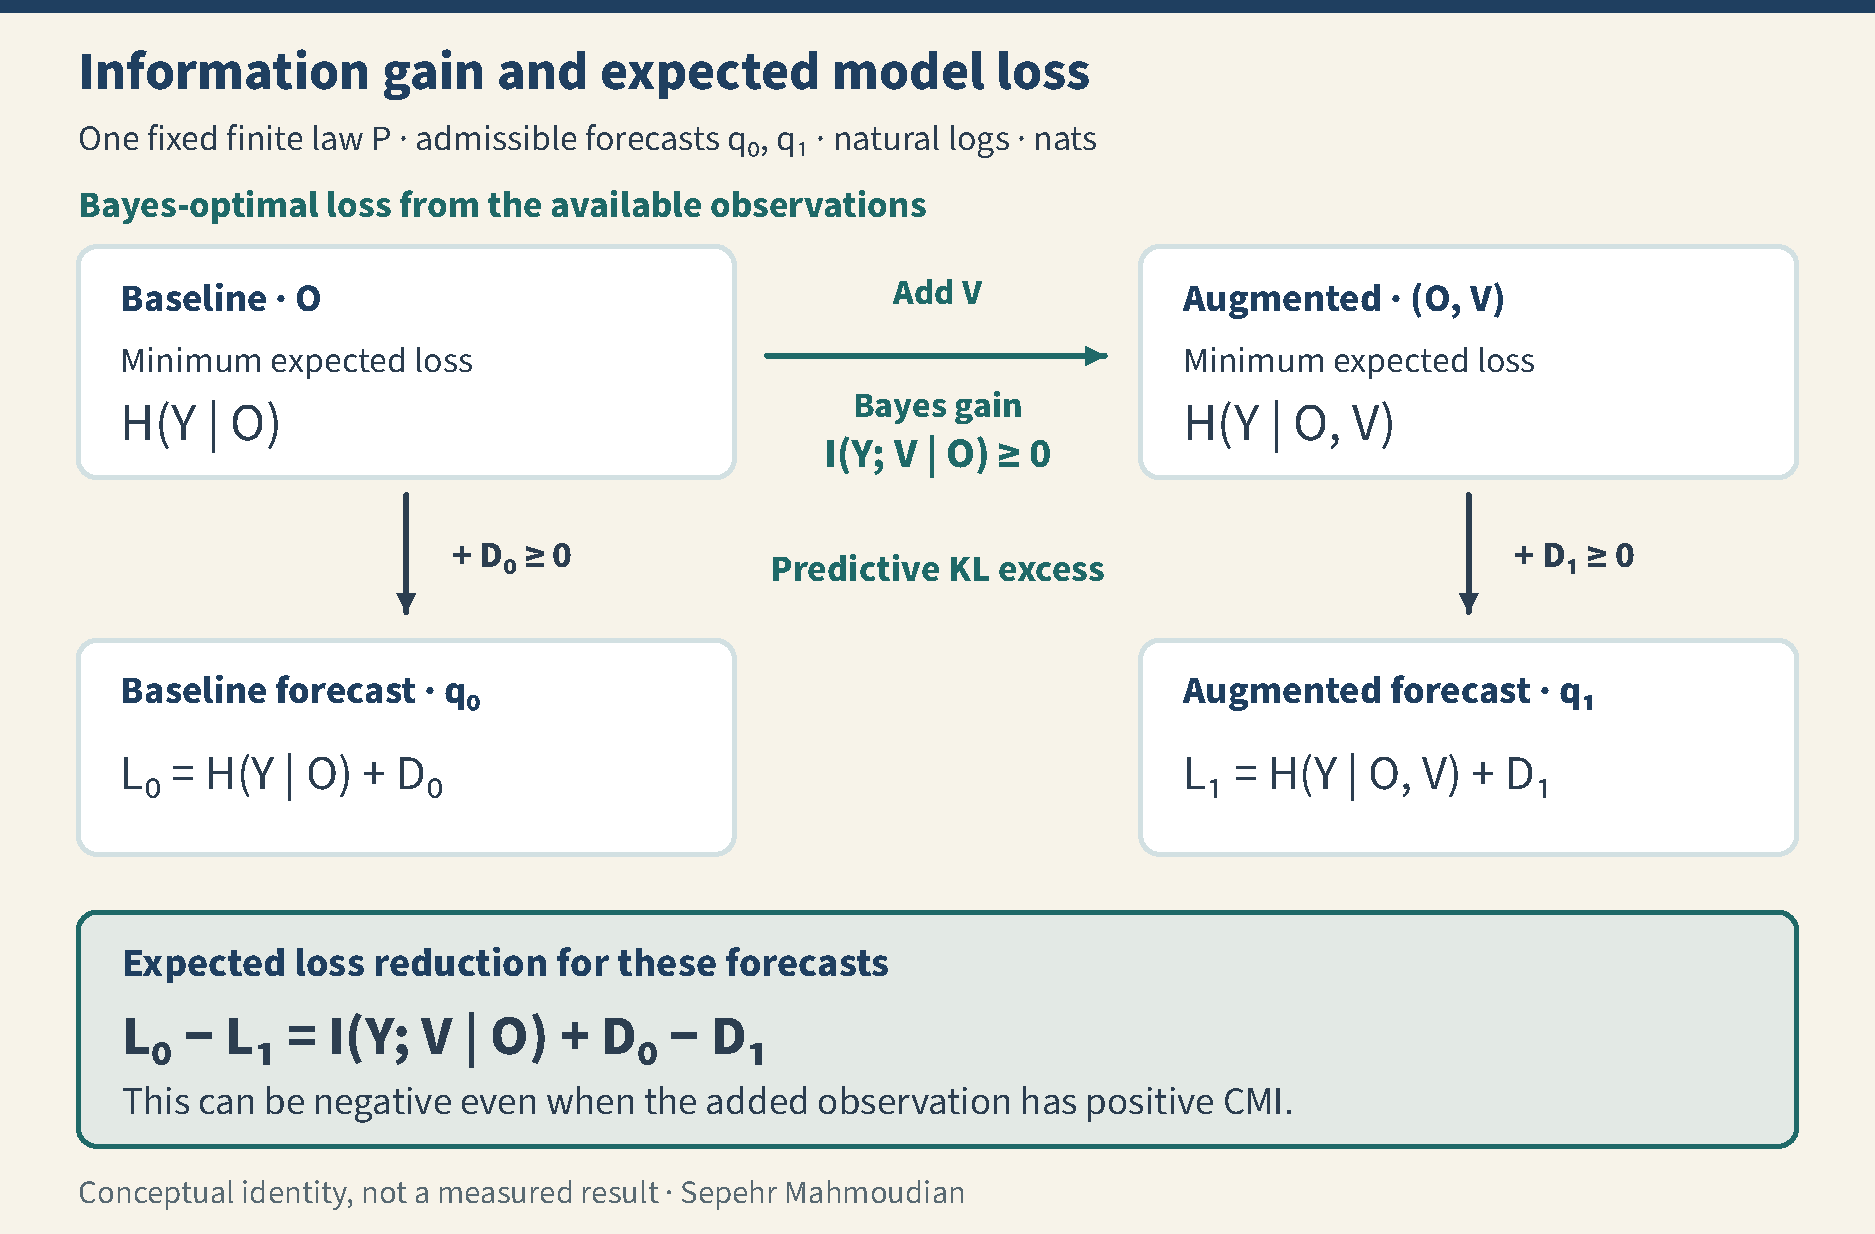
\includegraphics[width=160mm,height=\textheight,keepaspectratio,alt={Conceptual fixed-law expected-loss identity: the augmented observation lowers unrestricted Bayes loss by conditional information, while predictive KL excess determines the loss of supplied forecasts.}]{figures/loss-gap.pdf}
\caption{Conceptual fixed-law expected-loss identity: the augmented observation lowers unrestricted Bayes loss by conditional information, while predictive KL excess determines the loss of supplied forecasts.}
\end{figure}

\emph{Figure: Expected loss, not a measured model result. \(O\) is the baseline observation, \(V\) the added observation and \(Y\) the target; \(V\) is distinct from the synergy atom \(S\) in Section 2. Under one fixed finite law, \(L_0\) and \(L_1\) are the expected log losses of the admissible baseline and augmented forecasts. \(D_0\) and \(D_1\) are their nonnegative predictive KL excesses above the corresponding minimum expected losses. Each forecast is positive on supported target outcomes in every positive-probability observation fiber. Natural logs give nats. The Bayes gain \(I(Y;V\mid O)\) can be positive while \(L_0-L_1\) is negative.}

An augmented trained model can therefore perform worse even when the added observation contains information; its KL excess includes approximation, estimation and optimization errors. This identity does not establish a trained model's empirical loss, calibration or physical task value. If a forecast excludes a possible outcome, its ordinary expected log loss can be infinite and the finite-real subtraction above does not apply.

\par\Needspace{10\baselineskip}

\section{4. Exactly which atoms matter when sensors are unavailable?}\label{exactly-which-atoms-matter-when-sensors-are-unavailable}

Let \(M_i\in\{0,1\}\) indicate whether source \(i\) is available. Assume that the vector \(M=(M_1,M_2)\) is independent of the complete-data triple \((X_1,X_2,Y)\). The two mask bits may be correlated. Put \(p_{ij}=P(M_1=i,M_2=j)\).

Both compared Bayes predictors observe the same full mask. The baseline uses source 1 when present. The augmented predictor also uses source 2 when present. Both retain the same complete-data law, baseline availability and permitted context. In particular, withholding a recorded input does not change the behavior policy or the already recorded future target.

{\def\LTcaptype{none} % do not increment counter
\begin{longtable}[]{@{}
  >{\raggedright\arraybackslash}p{(\linewidth - 6\tabcolsep) * \real{0.1100}}
  >{\raggedright\arraybackslash}p{(\linewidth - 6\tabcolsep) * \real{0.2900}}
  >{\raggedright\arraybackslash}p{(\linewidth - 6\tabcolsep) * \real{0.2500}}
  >{\raggedright\arraybackslash}p{(\linewidth - 6\tabcolsep) * \real{0.3500}}@{}}
\toprule\noalign{}
\begin{minipage}[b]{\linewidth}\raggedright
Mask
\end{minipage} & \begin{minipage}[b]{\linewidth}\raggedright
Baseline observation
\end{minipage} & \begin{minipage}[b]{\linewidth}\raggedright
Additional source
\end{minipage} & \begin{minipage}[b]{\linewidth}\raggedright
Conditional loss reduction
\end{minipage} \\*
\midrule\noalign{}
\endhead
\bottomrule\noalign{}
\endfoot
\(00\) & No source & None & \(0\) \\*
\(10\) & \(X_1\) & None & \(0\) \\*
\(01\) & No source & \(X_2\) & \(I_2\) \\*
\(11\) & \(X_1\) & \(X_2\) & \(I_{12}-I_1\) \\*
\end{longtable}
}

Independence from complete data lets every row use the same \(P\). Average the four reductions, then substitute the reconstruction identities:

\[
\begin{aligned}
\Delta&=p_{01}I_2+p_{11}(I_{12}-I_1)\\
&=p_{01}(R+U_2)+p_{11}(U_2+S)\\
&=\boxed{p_{01}R+(p_{01}+p_{11})U_2+p_{11}S}.
\end{aligned}
\]

If the mask bits are also independent, with availabilities \(a=P(M_1=1)\) and \(b=P(M_2=1)\), then \(p_{01}=(1-a)b\) and \(p_{11}=ab\). Hence

\[
\boxed{\Delta=b[(1-a)R+U_2+aS].}
\]

The redundancy coefficient is the probability that source 2 can act as a backup. The unique coefficient is its availability. The synergy coefficient is joint availability. These are weights on signed allocations; an individual atom is not an independently realizable utility.

\begin{figure}
\centering
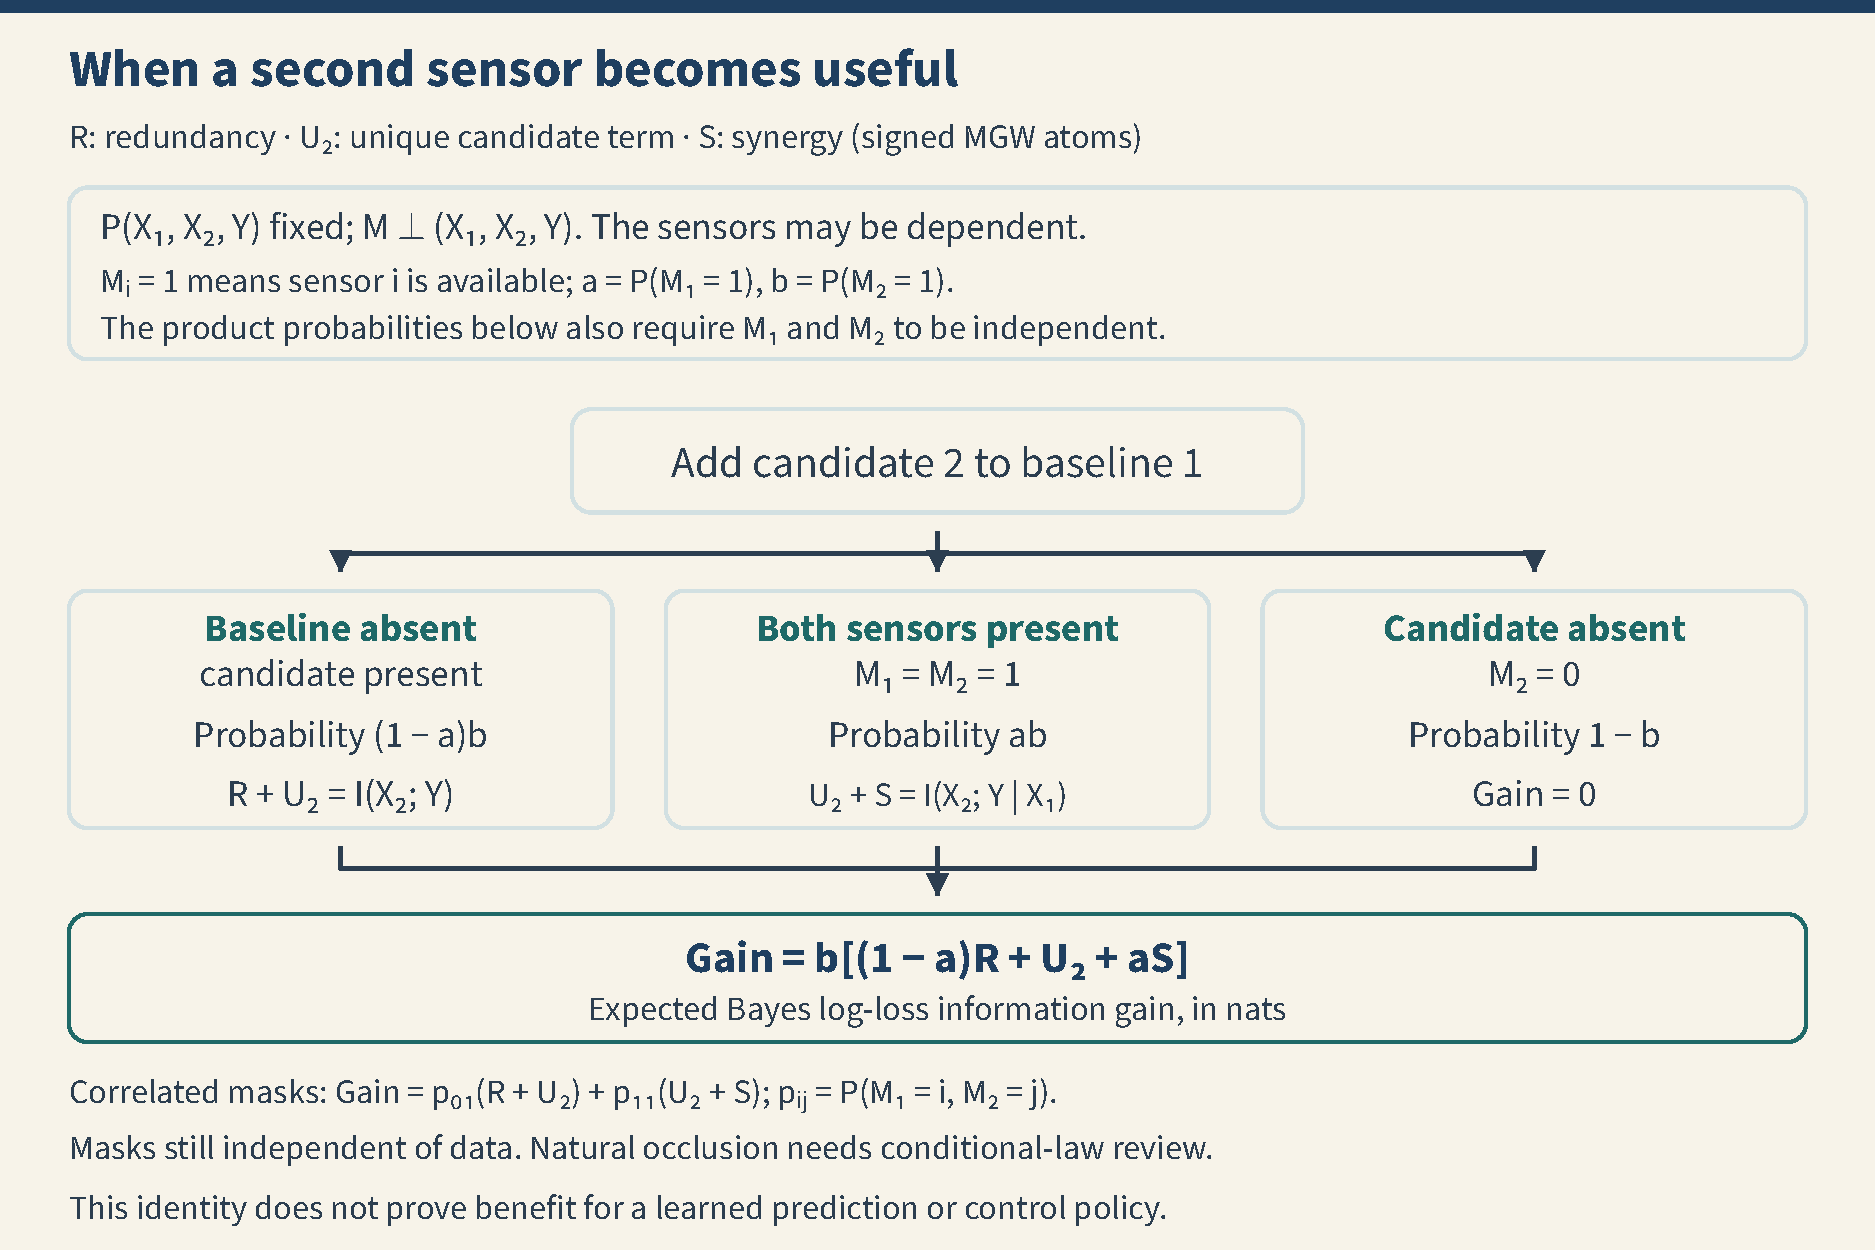
\includegraphics[width=160mm,height=\textheight,keepaspectratio,alt={Availability determines which signed combinations contribute to Bayes log-loss reduction. The complete-data law is fixed, and both predictors observe the same mask.}]{figures/availability-weighted-gain.pdf}
\caption{Availability determines which signed combinations contribute to Bayes log-loss reduction. The complete-data law is fixed, and both predictors observe the same mask.}
\end{figure}

The boundary cases provide useful checks. If \(b=0\), the gain is zero. If \(a=1\), it is \(b(U_2+S)\). If \(a=0\), it is \(b(R+U_2)\). For correlated failures, use \(p_{01},p_{11}\) directly. Marginal availabilities alone do not identify the backup benefit.

An acquisition cost can be included as \(\Delta-\lambda C\) only after defining expected incremental cost \(C\) and the conversion factor \(\lambda\) in nats per cost unit. Otherwise report the loss--cost trade-off without adding incompatible units.

\par\Needspace{10\baselineskip}

\section{5. Same synergy, different value: a complete calculation}\label{same-synergy-different-value-a-complete-calculation}

Let \(A,B,U\) be independent fair bits, so each of the eight triples has probability \(1/8\). Set the common target to \(Y=(A,B)\) and the baseline to \(X_1=A\). Compare three candidate second sources: independent noise \(U\), the complementary bit \(B\), and a duplicate of \(A\). The target, baseline and underlying world are unchanged across candidates.

Write \(\ell=\ln2\) and \(k=\ln(4/3)\). For candidate \(U\), the shared-exclusions event at an observed \((a,u)\) is \(\{A=a\}\cup\{U=u\}\). Its probability is \(1/2+1/2-1/4=3/4\). Conditional on the observed target \((a,b)\), the first event is certain. The local redundancy is therefore \(\ln(1/(3/4))=k\) at every supported state, so \(R=k\).

The baseline reveals one fair target bit: \(I_1=\ell\). Independent \(U\) reveals none: \(I_2=0\). Together they still reveal only \(A\): \(I_{12}=\ell\). Substitution gives

\[
R=k,\quad U_1=\ell-k,\quad U_2=-k,\quad S=k.
\]

For candidate \(B\), the union event again has probability \(3/4\) and is certain given \(Y\). Hence \(R=k\). Now \(I_1=I_2=\ell\) and \(I_{12}=2\ell\), giving

\[
R=k,\quad U_1=\ell-k,\quad U_2=\ell-k,\quad S=k.
\]

For duplicate candidate \(A\), the union event is just \(\{A=a\}\), with probability \(1/2\). Thus \(R=\ell\), and \(I_1=I_2=I_{12}=\ell\). All other atoms are zero.

{\def\LTcaptype{none} % do not increment counter
\begin{longtable}[]{@{}
  >{\raggedright\arraybackslash}p{(\linewidth - 10\tabcolsep) * \real{0.2600}}
  >{\raggedright\arraybackslash}p{(\linewidth - 10\tabcolsep) * \real{0.1000}}
  >{\raggedright\arraybackslash}p{(\linewidth - 10\tabcolsep) * \real{0.1200}}
  >{\raggedright\arraybackslash}p{(\linewidth - 10\tabcolsep) * \real{0.1200}}
  >{\raggedright\arraybackslash}p{(\linewidth - 10\tabcolsep) * \real{0.1000}}
  >{\raggedright\arraybackslash}p{(\linewidth - 10\tabcolsep) * \real{0.3000}}@{}}
\toprule\noalign{}
\begin{minipage}[b]{\linewidth}\raggedright
Candidate
\end{minipage} & \begin{minipage}[b]{\linewidth}\raggedright
\(R\)
\end{minipage} & \begin{minipage}[b]{\linewidth}\raggedright
\(U_1\)
\end{minipage} & \begin{minipage}[b]{\linewidth}\raggedright
\(U_2\)
\end{minipage} & \begin{minipage}[b]{\linewidth}\raggedright
\(S\)
\end{minipage} & \begin{minipage}[b]{\linewidth}\raggedright
Gain for independent masks
\end{minipage} \\*
\midrule\noalign{}
\endhead
\bottomrule\noalign{}
\endfoot
Independent \(U\) & \(k\) & \(\ell-k\) & \(-k\) & \(k\) & \(0\) \\*
Complement \(B\) & \(k\) & \(\ell-k\) & \(\ell-k\) & \(k\) & \(b\ell\) \\*
Duplicate \(A\) & \(\ell\) & \(0\) & \(0\) & \(0\) & \(b(1-a)\ell\) \\*
\end{longtable}
}

With \(a=0.8\) and \(b=0.9\), the gains are respectively \(0\), \(0.623832\) and \(0.124766\) nats, rounded to six decimals. The noise and complement have exactly equal synergy. Their unique atoms distinguish their added information. The duplicate has zero synergy but can be useful as a backup. If its failures always coincide with those of the baseline, \(p_{01}=0\) and that backup gain disappears.

\begin{figure}
\centering
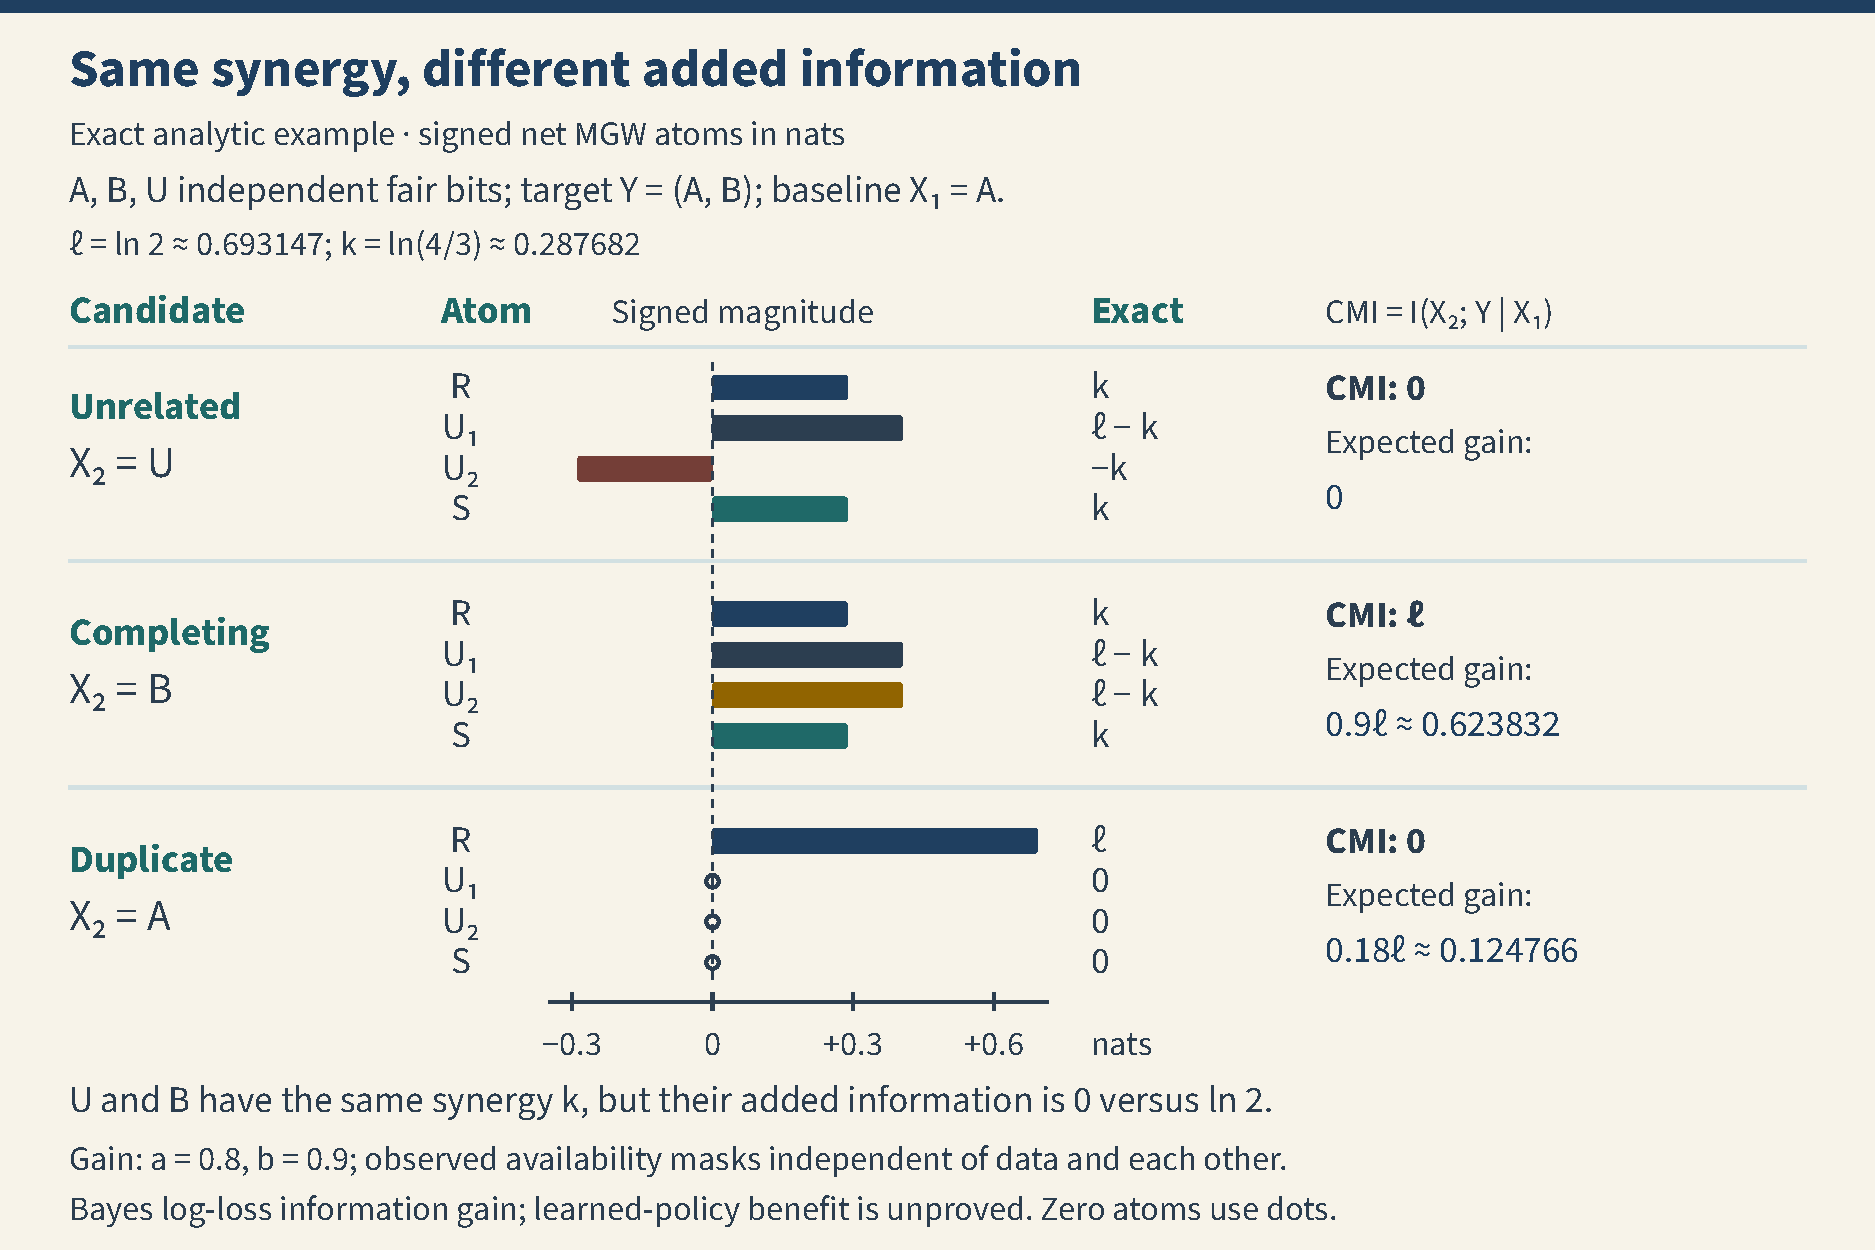
\includegraphics[width=160mm,height=\textheight,keepaspectratio,alt={Signed MGW atoms for noise, complement and duplicate candidates under one target law. Equal synergy does not imply equal added information. Bars crossing zero are retained.}]{figures/signed-atoms-and-sensor-value.pdf}
\caption{Signed MGW atoms for noise, complement and duplicate candidates under one target law. Equal synergy does not imply equal added information. Bars crossing zero are retained.}
\end{figure}

These are analytic controls, not sensor measurements. A target made of two ideal factors makes every probability explicit. It does not authorize copying an eventual outcome into a deployed feature. In real data, feature ancestry must exclude future reference labels. The \href{https://github.com/sepahead/pid-rs/blob/main/MATHEMATICAL_RESULTS_GUIDE.md}{fixed-world results guide} links the existing equal-synergy and target-copy formal work and its exact limits.

\par\Needspace{10\baselineskip}

\section{6. Natural occlusion changes the assumptions}\label{natural-occlusion-changes-the-assumptions}

Occlusion often depends on object position, scene geometry or viewpoint. It can therefore depend on \(Y\). The independence assumption of Section 4 must not be inferred from the word ``missing.'' Packet loss, detector rejection and absent annotations can also be value-dependent.

If both predictors observe the same full mask, condition on each positive-probability mask \(m\). Let \(P_m=P(\cdot\mid M=m)\). The exact replacement is

\[
\Delta=p_{01}I_{P_{01}}(Y;X_2)
+p_{11}I_{P_{11}}(Y;X_2\mid X_1).
\]

Each term uses its own conditional law. In general, one cannot substitute the unconditional MGW atoms. Information carried by the mask itself cancels because both comparators already observe it.

If the baseline sees only \(O_1=(M_1,\text{available }X_1)\) while the augmented predictor also sees \(M_2\), there is an additional term \(I(Y;M_2\mid O_1)\), followed by the added source-value information conditional on \(O_1,M_2\). It is not generally \(I(Y;M)\). If the baseline has no mask information at all, the information of the full available observation relative to the unconditional prior is

\[
I(Y;M)+\sum_mP(M=m)I_{P_m}(Y;X_m).
\]

Zero-probability mask strata contribute zero and need no conditional law. Rare positive strata may be impossible to estimate well from the available data.

\par\Needspace{10\baselineskip}

\subsection{Why separate independence checks are insufficient}\label{why-separate-independence-checks-are-insufficient}

Let \(Y,X\) be independent fair bits and set \(M=1\) exactly when \(X=Y\). Each pair \((Y,X)\) has probability \(1/4\). For either value of \(Y\), exactly one value of \(X\) gives \(M=1\), so \(P(M=1\mid Y)=1/2\). The same argument gives \(P(M=1\mid X)=1/2\). Thus \(M\) is independent of each variable separately, but not of their joint pair.

Give both predictors \(M\). The baseline receives no source reading, so its loss is \(H(Y\mid M)=\ln2\). When \(M=1\), the augmented predictor sees \(X=Y\) and its conditional loss is zero. When \(M=0\), it sees no reading and \(Y\) remains fair, so its conditional loss is \(\ln2\). Its expected loss is \((\ln2)/2\) and its gain is \((\ln2)/2\).

Yet unconditional \(I(Y;X)=0\). Multiplying this by availability would predict zero gain incorrectly. The correct gain is \(P(M=1)I_{P(\cdot\mid M=1)}(Y;X)=(\ln2)/2\). No extra mask information was hidden from the baseline. The source--target law changed within the available stratum. This exact negative control explains why the assumption concerns joint-law independence.

\textbf{First experiment.} Draw software masks independently of the complete recorded values, using fixed declared probabilities, and withhold the selected inputs from a fixed-policy recording. This makes availability exogenous by design and leaves the recorded target unchanged. Then test natural occlusion in a separate study with its conditional-law assumptions. Neither study alone establishes the effect of changing an active sensing or control policy.

If a common context \(C\) such as a task instruction is used, give it to both comparators. Apply the derivation within each context and average, provided \(M\) is independent of the complete data conditional on \(C\). Context-dependent mask probabilities must remain inside that average.

\par\Needspace{10\baselineskip}

\section{7. Two to four sources: a useful limit of the objective}\label{two-to-four-sources-a-useful-limit-of-the-objective}

Let \(M\) now denote a random available subset of \([n]=\{1,\ldots,n\}\), independent of the complete-data law. Write \(q_A=P(M=A)\). The expected Bayes log-loss reduction relative to the no-source predictor is

\[
J=\sum_{A\subseteq[n]}q_A I(Y;X_A),\qquad I(Y;X_\varnothing)=0.
\]

For each nonempty \(A\), reconstruction at the singleton antichain \(\{A\}\) gives

\[
I(Y;X_A)=\sum_{\alpha:\exists B\in\alpha,\ B\subseteq A}\pi_\alpha.
\]

Substitute this identity into \(J\) and interchange the two finite sums:

\[
\begin{aligned}
J&=\sum_Aq_A\sum_\alpha
\mathbf1\{\exists B\in\alpha:B\subseteq A\}\pi_\alpha\\
&=\sum_\alpha\left[\sum_Aq_A
\mathbf1\{\exists B\in\alpha:B\subseteq A\}\right]\pi_\alpha\\
&=\boxed{\sum_\alpha w_\alpha\pi_\alpha},\qquad
w_\alpha=P(\exists B\in\alpha:B\subseteq M).
\end{aligned}
\]

Every weight is between zero and one. Compute the probability of the union event; do not add the probabilities of overlapping matching branches. Mask bits need not be independent. The atoms are all from the same complete \(n\)-source law. A pairwise decomposition is not a substitute for the full lattice.

There are 4, 18 and 166 net atoms for two, three and four sources. This particular objective nevertheless depends only on the 3, 7 and 15 nonempty subset MI values. If two laws have the same subset MI values, every exogenous availability objective of this form agrees. Full PID adds an allocation, but no additional decision information for this exact oracle criterion.

This derivation uses only self-redundancy and lattice reconstruction. Its availability identity is therefore not exclusive to MGW; the signed numerical example in Section 5 is MGW-specific.

This is a useful negative conclusion: a PID-based optimizer of \(J\) must not claim an intrinsic advantage over an equivalent subset-MI optimizer. Finite estimators can differ in error and cost; such differences require measurement. Other PID questions remain possible, but they must specify what is learned beyond the subset-MI description.

\par\Needspace{10\baselineskip}

\subsection{Why pursue a three-source MGW decomposition?}\label{why-pursue-a-three-source-mgw-decomposition}

Three sources mean three declared input groups, not three sensor modalities or three coordinates. In the proposed study, \(X_1\) and \(X_2\) are fixed categorical features from two cameras, \(X_3\) is a fixed audio feature, and \(Y\) is a separately measured future outcome. The data-flow figure in Section 8 shows this representation boundary.

The additional question is explanatory: \textbf{how does the named MGW measure allocate target information across single sources and source combinations?} For example, it distinguishes a camera pair taken together versus audio from camera 1 versus the combination of camera 2 and audio. Let \(E_i\) mean that source \(i\) matches its observed value. Two different antichain indices use the events

\[
\alpha=\{\{1,2\},\{3\}\}:\qquad (E_1\cap E_2)\cup E_3,
\]

\[
\beta=\{\{1\},\{2,3\}\}:\qquad E_1\cup(E_2\cap E_3).
\]

Their Boolean definitions differ: on the hypothetical match pattern where only \(E_1\) holds, the first is false and the second is true. That pattern need not occur under a given source law. The events or their probabilities can coincide, for example with constant sources. Section 2 defines their target-dependent log ratios. Full three-source inversion then gives the 18 signed net atoms. An atom is not its cumulative event quantity, a separately computed two-source PID, or a nonnegative physical channel.

A predeclared diagnostic can compare the full-lattice signed atoms \(\pi_\alpha\) and \(\pi_\beta\), or specified sums of atoms, across visibility regimes and nominate a camera/audio representation or model ablation. Computing only the two cumulative event quantities would not require full PID3. That use still needs adequate stratum data, fixed source definitions, and matched prediction tests. Atom changes alone establish neither the model's use of a sensor nor a causal benefit. Subset MI and CMI can already detect decision-relevant joint dependence; detecting a three-way interaction does not by itself require full PID3.

The current availability-weighted Bayes objective needs only seven nonempty subset MI values for three sources. Thus full MGW is an optional explanatory analysis for that objective. A fusion model, sensor selector or training loop is not required to compute all 18 atoms. Use direct task loss and subset information when they answer the question.

The stable Rust three-source calculation already exists. The unfinished SxPID3 certificate program, indexed in the \href{https://github.com/sepahead/pid-rs/blob/main/MATHEMATICAL_RESULTS_GUIDE.md}{results guide}, seeks stronger assurance of its declared categorical outputs: source semantics, concrete formal definitions, certified arithmetic, compiled Rust correspondence and adversarial replay. As of 23 September 2026, none of its five complete programs A--E is closed. That assurance work matters when an allocation supports a scientific explanation; it does not establish estimator calibration or sensor benefit. Keep it separate from the practical benchmark, and from research-only continuous PID3, which uses a different functional.

\par\Needspace{10\baselineskip}

\section{8. From recorded measurements to a valid row}\label{from-recorded-measurements-to-a-valid-row}

The current ecosystem can record real simulator payloads. A payload record is not yet a target-specific statistical dataset. The proposed offline study needs the following explicit join.

\begin{figure}
\centering
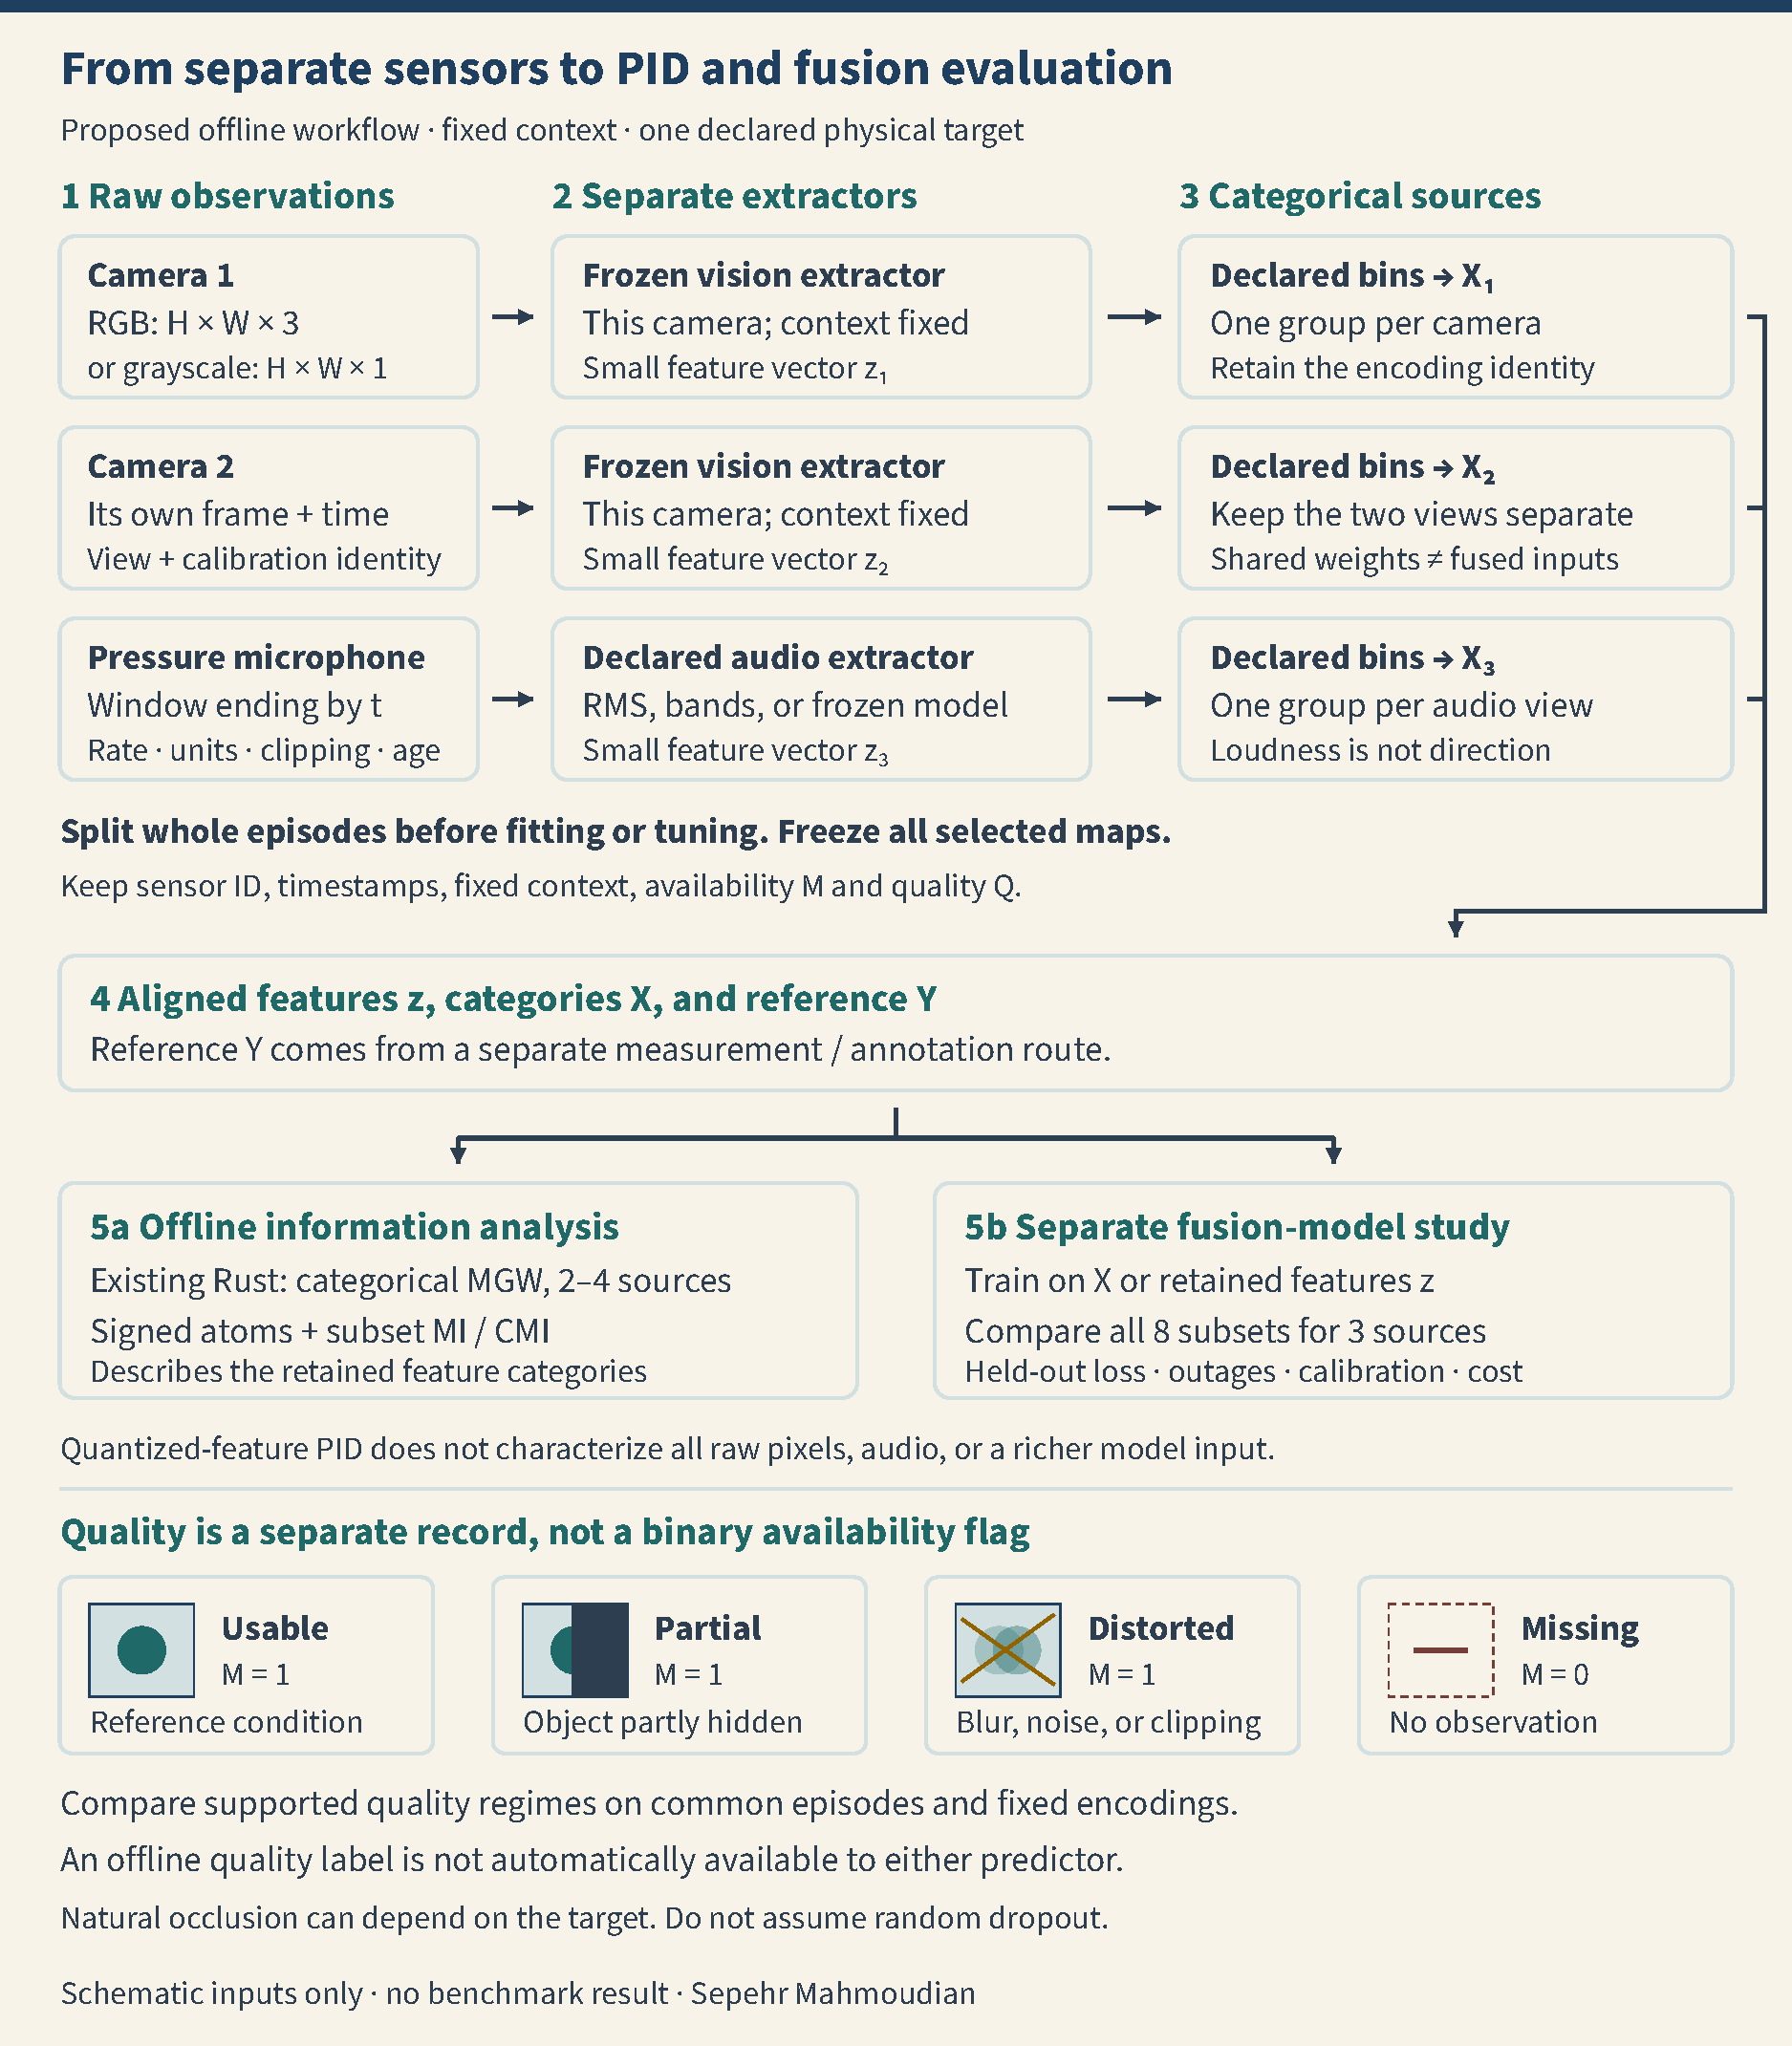
\includegraphics[width=160mm,height=\textheight,keepaspectratio,alt={Separate RGB or grayscale cameras and audio each produce a declared feature, then a categorical source. A separate reference supplies the target. PID and fusion-model evaluation answer different questions; the quality panel distinguishes partial, distorted and missing observations. The adapter and sensor study are proposed.}]{figures/sensor-data-to-evidence.pdf}
\caption{Separate RGB or grayscale cameras and audio each produce a declared feature, then a categorical source. A separate reference supplies the target. PID and fusion-model evaluation answer different questions; the quality panel distinguishes partial, distorted and missing observations. The adapter and sensor study are proposed.}
\end{figure}

\par\Needspace{10\baselineskip}

\subsection{Concrete source representation}\label{concrete-source-representation}

Start with two camera instances and one pressure microphone. An illustrative row at a predeclared time \(t\) could use:

\begin{itemize}
\tightlist
\item
  \(X_1\): a low-dimensional, training-frozen feature of camera 1 at or before \(t\), encoded in a fixed alphabet;
\item
  \(X_2\): the same declared type of feature for camera 2, with its own sensor identity and timestamp;
\item
  \(X_3\): a fixed pressure-window feature, for example RMS over a specified interval ending at \(t\), followed by training-fitted bins;
\item
  \(Y\): a future reference sector at \(t+\tau\), with fixed horizon \(\tau>0\), coordinate frame and bin edges.
\end{itemize}

For pressure samples \(p_1,\ldots,p_m\) in pascals, RMS is \(\sqrt{m^{-1}\sum_jp_j^2}\) pascals. RMS is only an example: it can discard direction, phase and frequency information needed by the task. It does not become range or object identity. A frozen audio feature must be judged against a no-audio baseline and alternative features.

Image features can likewise discard useful geometry. Record color space, orientation, calibration, instance, exposure/time policy and feature-model identity. A detector confidence is a model output, not a physical distance. No Gaussian prior is required for the resulting categorical PMF.

{\def\LTcaptype{none} % do not increment counter
\begin{longtable}[]{@{}
  >{\raggedright\arraybackslash}p{(\linewidth - 2\tabcolsep) * \real{0.3500}}
  >{\raggedright\arraybackslash}p{(\linewidth - 2\tabcolsep) * \real{0.6500}}@{}}
\toprule\noalign{}
\begin{minipage}[b]{\linewidth}\raggedright
Row field
\end{minipage} & \begin{minipage}[b]{\linewidth}\raggedright
Required interpretation
\end{minipage} \\*
\midrule\noalign{}
\endhead
\bottomrule\noalign{}
\endfoot
Run, episode, scene and landmark & Identifies one sampling unit and its physical context \\*
Sensor instance, frame and time window & Prevents accidental mixing of cameras or stale observations \\*
Feature and quantizer identity & Fixes what each categorical value means \\*
Availability and reason & Distinguishes withheld, not due, failed and unobserved values \\*
Target reference, frame, time and horizon & Binds an outcome independently of predictor features \\*
Action/policy and split identity & Prevents policy and training/evaluation leakage \\*
\end{longtable}
}

Do not encode ``not due'' as a zero-valued measurement. Choose either synchronized landmarks with all required sources, a declared causal holding/window rule, or an explicit missing-data study. These choices define different laws. Excluding incomplete rows can also select a different population.

The inspected native example advances six body ticks at 120 Hz. Camera periods two and three produce five total images, not six synchronized camera pairs. The microphone produces 133, 133, 134, 133, 133 and 134 pressure samples: 800 samples over 0.05 seconds. The retained two-camera-plus-audio capture contains 11 payloads and 1,542,400 bytes. These figures describe an engineering capture, not 800 independent observations or a PID evaluation. The native model's physical calibration and any real-world transfer remain separate questions.

\par\Needspace{10\baselineskip}

\subsection{Fit, evaluate and preserve the estimand}\label{fit-evaluate-and-preserve-the-estimand}

Split complete episodes before fitting features, quantizers or predictors. Fit all choices on training episodes, freeze them, and apply them to evaluation episodes. Report bin edges, alphabet sizes, occupancy, clipping/out-of-range behavior and rejected rows. An empirical zero cell is not evidence of a population zero. Training and evaluation occupancy must not be silently pooled.

If every source and the target has eight categories, three sources allow \(8^4=4096\) complete cells; four allow \(8^5=32768\). This explains why raw high-dimensional inputs cannot simply be discretized finely. More bins can reduce representation bias while making population estimation worse. Report sensitivity to prespecified coarser encodings. Selecting the best encoding on the final test data invalidates an ordinary held-out comparison.

Hyperbolic latent coordinates do not remove this problem. Quantizing them produces a categorical representation with a declared geometry-dependent encoder. It does not establish a hyperbolic continuous PID estimator or avoid the joint-alphabet cost. Continuous and manifold-supported inputs need their own support and metric analysis.

\par\Needspace{10\baselineskip}

\subsection{Exactly what enters PID for cameras and audio}\label{exactly-what-enters-pid-for-cameras-and-audio}

The runtime estimator receives matrices of categorical labels, not an image file, waveform or neural network. The camera/audio adapter below is a proposed implementation contract. The completed real-data example in this report uses office measurements; no end-to-end camera/audio PID experiment is claimed.

For one camera, let \(H\) and \(W\) denote image height and width in the image-shape notation used here. An RGB frame has shape \(H\) by \(W\) by three channels; a grayscale frame has one intensity channel. Preserve color space, channel order, exposure and pixel scaling. Grayscale conversion discards color and therefore changes the observed representation. It can be a separately tested input choice, not an equivalent replacement for RGB. Resizing, crops and image normalization also belong to the declared feature map.

Encoding every pixel as a categorical coordinate is mathematically possible, but it is not the proposed first estimator. An 8-bit grayscale frame already has up to \(256^{HW}\) possible intensity patterns. When almost every frame is a distinct state, an empirical table can identify individual recorded rows without establishing useful population prediction. A smaller feature representation trades away information to make repeated states and a defensible statistical study possible. Its loss of information must remain explicit.

A frozen vision extractor maps each camera's own pre-target frames to a small feature vector. This can be a geometric feature with calibrated meaning, a detector output, or a learned representation. A detector probability is a prediction, not ground-truth presence, distance or identity. A dense latent with hundreds of coordinates is not automatically an estimable categorical source: its joint alphabet can be prohibitive. Begin with a small, meaningful feature and report what it discards.

A pressure microphone supplies time-indexed samples with declared units and sampling rate. A fixed window ending by the prediction time can be summarized by RMS, band energies, or a frozen audio encoder. State window length, sample rate, channel count, filtering, resampling, normalization and clipping policy. Band energy preserves different information from a single loudness value; neither a scalar energy nor single-microphone RMS establishes direction or object identity. An array-derived direction estimate needs the microphone geometry, synchronization and a separate validated localization method. Missing samples and silence are different observations.

Each sensor must first be transformed separately. Shared network weights across two cameras are permissible if each output depends only on its own camera and declared common context. Record that context and give the comparators the same permitted access to it. If \(X_i=f_i(\mathrm{camera}_i,C)\) uses shared context \(C\), the unconditional PID can include information carried by \(C\). Equal predictor access does not remove that information from the PID. For a sensor-specific interpretation, hold \(C\) fixed or compute and report the finite-law decomposition within each supported context stratum. An average of those decompositions is a conditional analysis, not the unconditional decomposition. If a purported camera-1 feature already consumes camera 2 or audio, the source labels no longer represent separate sensors. A fused network output is not a third independent sensor.

\par\Needspace{10\baselineskip}

\subsection{An explicit illustrative row and fusion experiment}\label{an-explicit-illustrative-row-and-fusion-experiment}

Consider a proposed single-object presence forecast with target \(Y\in\{0,1\}\) at a fixed future horizon. This is one possible study; the future-sector task above uses a different target alphabet and needs its own evaluation. Obtain \(Y\) from a separately justified reference. Train or select the three feature-extraction paths using development data only. Record each model version and weight identity, its pretraining and fine-tuning data, and any overlap with evaluation episodes or reference labels. Frozen weights alone do not establish an uncontaminated evaluation. Freeze the selected maps before outer evaluation:

\begin{itemize}
\tightlist
\item
  one vision extractor applied separately to camera 1 and camera 2;
\item
  one audio extractor applied to the pre-target pressure window.
\end{itemize}

For this illustration, each extractor outputs a scalar event score in \([0,1]\). A score need not be calibrated to serve as a declared source feature; calibration is separately tested if the score is used as a predictive probability. Choose four fixed bins in advance: \([0,1/4)\), \([1/4,1/2)\), \([1/2,3/4)\) and \([3/4,1]\). This fixed map is an alternative to training-fitted edges, not a claim about the fitted quantizer's edges. Handle invalid or unavailable outputs through an explicit status rule rather than putting them in the lowest bin.

{\def\LTcaptype{none} % do not increment counter
\begin{longtable}[]{@{}
  >{\raggedright\arraybackslash}p{(\linewidth - 4\tabcolsep) * \real{0.2800}}
  >{\raggedright\arraybackslash}p{(\linewidth - 4\tabcolsep) * \real{0.3200}}
  >{\raggedright\arraybackslash}p{(\linewidth - 4\tabcolsep) * \real{0.4000}}@{}}
\toprule\noalign{}
\begin{minipage}[b]{\linewidth}\raggedright
Field
\end{minipage} & \begin{minipage}[b]{\linewidth}\raggedright
Illustrative value
\end{minipage} & \begin{minipage}[b]{\linewidth}\raggedright
Meaning
\end{minipage} \\*
\midrule\noalign{}
\endhead
\bottomrule\noalign{}
\endfoot
Camera 1 score & \(0.72\) & Its separate extractor output; category \(X_1=2\) \\*
Camera 2 score & \(0.41\) & Its separate extractor output; category \(X_2=1\) \\*
Audio score & \(0.68\) & Its separate window extractor output; category \(X_3=2\) \\*
Future reference & \(Y=1\) & An independently sourced outcome after the feature windows \\*
\end{longtable}
}

These numbers are invented to explain the interface; they are not recorded measurements or benchmark results. One valid row enters the categorical matrices as source labels \((2,1,2)\) and target label \(1\). Many aligned rows produce counts for a nominal \(4^3\times2=128\)-cell joint PMF. The stable three-source calculation then reports the 18 averaged MGW atoms on that represented empirical law. The two-camera calculation has four atoms; adding a fourth source gives 166. Report occupied cells, counts and source provenance as well as atoms. The six-tick capture described above is an engineering fixture and is too short to substitute for this repeated-episode study.

The \textbf{fusion predictor is separate}. Feed it the permitted sensor features, quality metadata and availability mask, and train it to predict the reference outcome. Compare all eight subsets of three sources, including the no-sensor baseline, on identical held-out episodes. If PID uses quantized scores but the predictor uses unquantized scores, say so: the PID concerns a coarsening of the predictor's inputs. Compare a predictor on the same categories when a direct correspondence is needed. If a predictor consumes full images or audio embeddings, a scalar-score PID does not characterize all of its available input information.

Three analyses must remain distinct:

\begin{enumerate}
\def\labelenumi{\arabic{enumi}.}
\tightlist
\item
  \textbf{Sensor-feature PID:} sources are separate sensor representations and the target is the physical reference. It asks what information those representations retain.
\item
  \textbf{Representation PID:} sources are explicitly selected neural layers, branches or bottlenecks, with a declared target. It asks what those internal variables retain. State every input each branch has already consumed; post-fusion branches cannot automatically be interpreted as separate camera or audio sources.
\item
  \textbf{Model-use evaluation:} measure predictions, calibration and matched ablations of the fitted fusion model. It asks what the model actually exploits. Neither of the first two information tables alone establishes this use.
\end{enumerate}

Taking the model's output as the PID target is another valid but different descriptive question: it concerns information about the model's decision, not information about physical truth. A wrong or shortcut-based model can still have a strong decomposition relative to its own output. Keep the reference-target and model-output analyses separately named and never use one as validation of the other.

\par\Needspace{10\baselineskip}

\subsection{Where the offline analysis changes a decision}\label{where-the-offline-analysis-changes-a-decision}

Offline means that the analysis runs on a retained dataset after capture. It can guide the next engineering experiment without running inside a robot's control loop. The current useful output is a report: the row and target contract, subset information, signed MGW atoms, predictor losses, data limitations and measured costs. It is not a trained controller or a sensor-placement command.

{\def\LTcaptype{none} % do not increment counter
\begin{longtable}[]{@{}
  >{\raggedright\arraybackslash}p{(\linewidth - 4\tabcolsep) * \real{0.2800}}
  >{\raggedright\arraybackslash}p{(\linewidth - 4\tabcolsep) * \real{0.3200}}
  >{\raggedright\arraybackslash}p{(\linewidth - 4\tabcolsep) * \real{0.4000}}@{}}
\toprule\noalign{}
\begin{minipage}[b]{\linewidth}\raggedright
Development stage
\end{minipage} & \begin{minipage}[b]{\linewidth}\raggedright
Useful output and decision
\end{minipage} & \begin{minipage}[b]{\linewidth}\raggedright
Evidence needed beyond PID
\end{minipage} \\*
\midrule\noalign{}
\endhead
\bottomrule\noalign{}
\endfoot
Data preparation & An aligned table identifies rejected joins, stale inputs and missing reference outcomes. Decide whether to repair capture or collect more data. & Clock, unit, calibration, transport and association checks. Atoms do not perform these checks. \\*
Label engineering & Target lineage and disagreement records identify cases for reference review. Decide whether the outcome definition or annotation needs correction. & Reference measurements or adjudication. Dependence with a label cannot certify that label. \\*
Feature engineering & Compare a few frozen encodings of the same sensor groups. Decide which representation deserves a matched predictor experiment. & Training-only fitting, common evaluation rows, direct task loss and representation sensitivity. Bins define a different estimand from raw data. \\*
Fusion-model design & Compare available information with the information a fitted model exploits. Decide which subset or failure regime needs an ablation. & Matched model tests. PID of inputs alone does not show the internal use of those inputs. \\*
Tuning & Report signed allocation beside validation loss for a declared candidate family. Choose parameters inside the development splits. & A final untouched evaluation and a selection-aware uncertainty design. Maximizing an attractive atom on the test set is tuning on the test set. \\*
Placement and acquisition & Explain shortlisted portfolios and nominate a new collection experiment. & Candidate-location data or a justified observation model, geometry, costs, failures and held-out task utility. An unobserved camera location has no measured joint law. \\*
Training and policy creation & Form a specific objective or architecture hypothesis for later testing. & An implemented learner, support and gradient conditions, matched training baselines and closed-loop evaluation for control claims. \\*
Integrity and monitoring & Inspect whether a predeclared sensor relationship changes across retained operating regimes. & Fault labels, benign-shift controls and calibrated alerts. A changed atom does not distinguish tampering, misalignment, weather or an ordinary distribution change. \\*
\end{longtable}
}

The preparation and label outputs are valuable even when PID is omitted. Use MGW only when its allocation answers a stated question beyond the direct scores. For example, the equal-synergy calculation in Section 5 explains why a synergy-only ranking confuses independent noise with useful complementary information. If direct task loss already settles the engineering choice and the allocation has no further explanatory role, stop there.

\par\Needspace{10\baselineskip}

\subsection{Label provenance is not statistical independence}\label{label-provenance-is-not-statistical-independence}

An independent reference means that the label has a separately justified measurement or annotation route. It does \textbf{not} mean that \(Y\) is statistically independent of the sensors: that would remove the predictive relationship under study. For each target retain its instrument or annotator, physical meaning, coordinate frame, timestamp, horizon, ambiguity and adjudication rule. A simulator state can be a reference for a simulation study; this does not establish a real-world measurement model.

PID does not generate ground truth. It can support a request to inspect selected cases, but a large atom can reflect a useful signal, leakage or a coding choice. A small atom can reflect a poor feature, little variation or insufficient data. Confirm label errors with the reference system. Retain unresolved cases and report the selection introduced by excluding them. For multi-object recordings, match each feature and reference to the same physical object under a declared association rule; an association algorithm's prediction must not silently become its own truth label.

\par\Needspace{10\baselineskip}

\subsection{Partial visibility and distorted observations}\label{partial-visibility-and-distorted-observations}

Availability is not a quality scale. Distinguish a missing observation from an available but partial or degraded one. A camera can return a valid frame with most of an object hidden; a microphone can return pressure samples dominated by wind. Preserve both the availability mask \(M\) and a declared quality/context variable \(Q\). Examples of \(Q\) are a specified blur level, clipping fraction, frame age or an annotated occlusion category. Quality measurements and annotations can themselves be uncertain.

{\def\LTcaptype{none} % do not increment counter
\begin{longtable}[]{@{}
  >{\raggedright\arraybackslash}p{(\linewidth - 4\tabcolsep) * \real{0.2800}}
  >{\raggedright\arraybackslash}p{(\linewidth - 4\tabcolsep) * \real{0.3200}}
  >{\raggedright\arraybackslash}p{(\linewidth - 4\tabcolsep) * \real{0.4000}}@{}}
\toprule\noalign{}
\begin{minipage}[b]{\linewidth}\raggedright
Condition
\end{minipage} & \begin{minipage}[b]{\linewidth}\raggedright
Preserve in the data
\end{minipage} & \begin{minipage}[b]{\linewidth}\raggedright
Compare on common episodes
\end{minipage} \\*
\midrule\noalign{}
\endhead
\bottomrule\noalign{}
\endfoot
Partial field of view or occlusion & Sensor pose, region/window, reference visibility category and annotation uncertainty & Single-view and fused prediction in each supported visibility regime \\*
Blur, low light or noise & Exposure, declared corruption rule and scale, feature identity and target reference & Clean and degraded inputs, calibration and task loss across severity \\*
Audio clipping or interference & Units, window, gain, clipping fraction and interference conditions & Camera-only, audio-only and fused predictions; retain no-audio controls \\*
Delay or stale frames & Capture and arrival times, clock uncertainty and causal age rule & Delay-aware baseline and fusion under measured delays; never join future frames \\*
Calibration or alignment error & Calibration revision, coordinate frame and known perturbation & Physical prediction error and sensor consistency before interpreting atoms \\*
\end{longtable}
}

First restrict the comparison to a declared availability stratum with all compared source values observed, or define a separate missing-data estimand. In that fixed row population, for finite \(Q\), an analysis within a quality stratum uses the conditional law \(P(X_1,\ldots,X_n,Y\mid Q=q)\) when \(P(Q=q)>0\). Compute MGW on that specified conditional law and retain its signed atoms. Here each \(X_i\) denotes the actually observed, possibly degraded feature, not an unavailable clean signal. Pooling all qualities answers a different question. Target prevalence and scene difficulty can also differ across strata, so an atom difference between strata is descriptive evidence, not a causal effect of degradation. Small strata can be too sparse to interpret; report counts and abstain where the evidence is insufficient. Keep the feature maps and alphabet fixed across strata when comparing allocation; otherwise report the representation change explicitly.

If \textbf{both predictors observe \(Q\)}, the unrestricted Bayes gain from adding \(X_2\) is \(I(Y;X_2\mid X_1,Q)\). Apply Section 3 within each positive-probability value of \(Q\) and average. For two-source conditional MGW, this is the corresponding average of \(U_2(q)+S(q)\), not synergy alone. This is a handwritten application of the same finite-law identities, not a newly checked formal result. If quality is available only to an offline annotator, this describes an oracle-quality comparison. Evaluate the deployable model with its actual inputs instead. If \(Q\) is computed from the added sensor and cannot be obtained without it, giving \(Q\) to the baseline already supplies part of that sensor's information. The displayed gain then measures residual value after that quality signal, not total acquisition value. For an operational comparison, give each predictor only the quality or metadata it can actually obtain and count the information and cost of any additional quality signal. Estimating quality from the same camera is an explicitly defined feature, not independent evidence of quality.

Controlled corruption and natural degradation need different interpretations. For a declared experiment, apply a frozen corruption mechanism at stated severities, retain the original labels only when the mechanism leaves their physical meaning unchanged, and keep all variants of an episode in one split. Independent random corruption can test a controlled robustness question. Natural occlusion may depend on target location, action or weather; conditioning or dropping those rows changes the law and can introduce selection effects. A complete-data random-dropout formula does not automatically apply. Section 6 gives the relevant mask boundary.

The practical use is to find supported regimes in which a sensor combination retains information but the fitted fusion model fails, or in which the represented inputs contain little additional information at all. These findings nominate different follow-ups: improve the predictor, improve the feature, or collect a better observation. They do not uniquely diagnose the cause. Compare loss, missed detections, false alarms, calibration and latency alongside PID. No conditional-stratum adapter, corruption benchmark or qualified degradation monitor is added by this exposition; those remain implementation and evaluation work.

\par\Needspace{10\baselineskip}

\subsection{A complete preparation-to-decision sequence}\label{a-complete-preparation-to-decision-sequence}

\begin{enumerate}
\def\labelenumi{\arabic{enumi}.}
\tightlist
\item
  \textbf{Define the question.} For example, test whether two camera features plus an audio feature predict a later object sector more reliably than one camera. Specify the sector frame, prediction horizon, feature windows, eligible episodes, source groups and useful loss improvement before looking at results. This is a proposed embodied study, not a completed dataset.
\item
  \textbf{Build causal rows.} At each declared landmark, use only measurements available by that time. Preserve raw record identities and the exact join tolerance. Report unmatched references, late packets, reused frames and exclusions. Audio samples inside one window are inputs to one feature, not independent PID rows.
\item
  \textbf{Separate development from evaluation.} Assign whole episodes, missions, sites or time periods to splits that match the intended transfer claim. Fit encoders, scalers, bins and predictors on training data; choose hyperparameters on validation data. Freeze the selected pipeline before the final test. All variants of one episode stay together.
\item
  \textbf{State the row law.} The current row API gives each admitted row equal mass. Long episodes then contribute more mass if they supply more rows. To study equally weighted episodes, use a justified landmark design or a separately implemented weighted-law route; do not claim that the row API performs episode weighting. Exact empirical-table identities do not require IID rows. Population inference does require a justified sampling and dependence model.
\item
  \textbf{Check the categorical object.} Retain the frozen alphabet and out-of-range rule, occupied cells, cell counts, target frequencies and missingness by regime. No Gaussian prior or independence between sensor sources is required for the categorical functional. An observed empty cell is not a population zero, and a large row count is not an independent-sample count.
\item
  \textbf{Compare direct outcomes first.} Evaluate every relevant subset on common outer rows with the same target. Record proper loss, calibration, relevant task metrics, availability and cost. Keep fixed-model outages separate from retrained subset models. Then report the MGW allocation for a preselected question, retaining negative atoms.
\item
  \textbf{Make a bounded decision.} Keep a representation or nominate a collection experiment only when its stated criterion is met. Preserve no-benefit and unstable-encoding results. If a new target, grouping or feature is chosen after inspection, treat it as development and obtain a new confirmation dataset before a confirmatory claim.
\end{enumerate}

Repeated landmarks within one episode can remain dependent. The episode bound in Section 9 has its own independence and probability-floor premises; it is not granted by executing this sequence. Block resampling also needs a valid dependence model. A deterministic empirical PID evaluation is not automatically an unbiased or calibrated population estimate.

\par\Needspace{10\baselineskip}

\subsection{Recorded measurements: information can increase while prediction gets worse}\label{recorded-measurements-information-can-increase-while-prediction-gets-worse}

A completed, narrower example uses recorded office light in lux, CO₂ in ppm and a same-time binary occupancy label. Its reference provenance, input statistics, raw-row examples and numerical checks are retained in the \href{https://github.com/sepahead/pid-rs/blob/main/audit/evidence/real-occupancy-sensors-example-2026-09-08.md}{office-sensor study}. The study cites the UCI provider, which describes photograph-derived occupancy labels. This example is classification of recorded occupancy, not future robot-state prediction.

Four bins for each source were fitted on 8,143 training rows and frozen. The later recording has 9,752 rows. Its nominal source-target alphabet has \(4\times4\times2=32\) cells; 16 are occupied, four occupied cells contain fewer than five rows, and the smallest contains one row. Those are input statistics, not a population-support guarantee. The records are time series from one office; the comparison does not establish independent samples or transfer to other buildings.

Write \(A\) for the light category and \(B\) for the CO₂ category. Each fixed predictor was fitted from training counts: in a source cell with \(n\) rows and \(n_1\) occupied outcomes, it assigns occupancy probability \((n_1+1)/(n+2)\). Thus an unseen training cell predicts \(1/2\). The test recording determines the empirical evaluation law, not the fitted prediction rule.

The retained test values, rounded to nine decimals, are

\[
\begin{aligned}
I(Y;B\mid A)&\approx0.001558012,\\
L(q_A)&\approx0.047443051,\\
L(q_{AB})&\approx0.050762019.
\end{aligned}
\]

All information is in nats; loss is mean nats per row. The positive conditional information says that the Bayes predictor for this empirical test law can gain from \(B\). The fixed training-fitted predictor instead has gain

\[
L(q_A)-L(q_{AB})\approx-0.003318968.
\]

Section 3 explains the sign. The \href{https://github.com/sepahead/pid-rs/blob/main/audit/evidence/occupancy-fixed-predictor-loss-decomposition-2026-09-10.md}{recorded loss-gap analysis} reports predictive excess losses of approximately \(D_A=0.014359564\) and \(D_{AB}=0.019236545\). Their difference is \(-0.004876981\); adding the positive information gain gives approximately \(-0.003318969\). The last-digit difference comes from the displayed rounding. The augmented model's larger excess loss outweighs the available-information gain. This identity does not identify which part of that excess arises from estimation, approximation or optimization.

The MGW allocation gives another useful warning: its added-source unique atom is approximately \(-0.178691053\) and synergy is \(0.180249065\). Their sum is \(0.001558012\). Keeping synergy alone would hide nearly complete cancellation. The engineering response is to inspect the representation, sparse cells and predictor fit, then test any correction on new data. These recorded results do not show that PID improved the model or caused its failure. Reusing this already inspected recording for a new choice would require a new evaluation boundary.

\par\Needspace{10\baselineskip}

\section{9. A falsifiable first study and its statistics}\label{a-falsifiable-first-study-and-its-statistics}

The first study is offline future-outcome prediction under controlled camera withholding. Keep all variants of one physical episode together. Freeze the target, features, mask probabilities, learners, tuning budgets, subgroup roster and useful improvement margin before evaluating untouched episodes.

For three sources, evaluate all eight masks. Compare a context-only predictor, the three single-source predictors, the source subsets, and the complete-source predictor. Distinguish two interventions:

\begin{itemize}
\tightlist
\item
  \textbf{Fixed-model outage:} remove an input at evaluation from a model trained by a declared masking procedure. This tests its robustness.
\item
  \textbf{Retrained subset:} train each subset model separately with a matched tuning budget. This tests how well each allowed sensor set can support prediction.
\end{itemize}

The primary metric is the declared task loss. Report direct subset MI/CMI and the full signed MGW result as diagnostics, with estimator assumptions. A win against synergy alone is not evidence that PID improves on these stronger comparators.

\par\Needspace{10\baselineskip}

\subsection{One conservative finite-sample rule}\label{one-conservative-finite-sample-rule}

Condition on the frozen training/design artifacts. Assume an integer \(N\geq1\) independent evaluation episodes from the same declared law. Within an episode, frames and mask variants may be dependent. Define one episode loss by a prespecified weighted average with nonnegative weights summing to one.

Require every predictor probability to be at least \(\varepsilon>0\) on the finite target alphabet, with \(\varepsilon\leq1/|\mathcal Y|\). A specified normalized smoothing rule is needed; clipping each coordinate independently need not preserve a PMF. For example, with \(d=|\mathcal Y|\) and a fitted PMF \(\widetilde q\), set \(q_\varepsilon(y\mid o)=(1-d\varepsilon)\widetilde q(y\mid o)+\varepsilon\). Its entries sum to one and each is at least \(\varepsilon\). Each log loss is in \([0,B]\), where \(B=\ln(1/\varepsilon)\). Such smoothing generally leaves KL excess above the unrestricted Bayes entropy; the bounded-loss evaluation is not an assertion that the entropy optimum is attained.

Let \(D_i\) be the baseline episode loss minus augmented episode loss, after averaging all masks with their fixed weights. Then \(-B\leq D_i\leq B\). If \(B=0\), the admitted target is a singleton and all losses and differences are zero; no concentration estimate is needed. For \(B>0\) and \(t>0\), Hoeffding's classical bounded-variable inequality gives

\[
P\!\left(\overline D-E D\geq t\right)
\leq\exp\!\left(-\frac{Nt^2}{2B^2}\right).
\]

Set the right side equal to \(\delta\in(0,1)\) and solve for \(t\):

\[
t=B\sqrt{\frac{2\ln(1/\delta)}{N}}.
\]

Thus, with probability at least \(1-\delta\),

\[
E D\geq\overline D-B\sqrt{\frac{2\ln(1/\delta)}{N}}.
\]

Require this lower bound to exceed the predeclared useful margin before asserting a useful mean improvement under this evaluation law. A one-sided error allowance at most \(w>0\) has sufficient planning size \(N\geq2B^2\ln(1/\delta)/w^2\). This bound can be expensive and conservative; it is not a promise that the available capture meets the assumptions. The source is \href{https://doi.org/10.1080/01621459.1963.10500830}{Hoeffding, \emph{Probability Inequalities for Sums of Bounded Random Variables}}.

All eight masks of an episode still give one \(D_i\), not eight independent samples. Reused scenes, overlapping trajectories, adaptation, optional stopping and selective successful-capture inclusion require further design. For several selected primary comparisons, allocate the error budget across them or use a separately justified simultaneous procedure. This bound concerns predictive loss, not PID estimator calibration.

\par\Needspace{10\baselineskip}

\section{10. Learning, planning and physical intelligence}\label{learning-planning-and-physical-intelligence}

A realistic first training objective is ordinary masked prediction:

\[
\mathcal L(\theta)=\sum_Aq_A\,
E[-\ln q_\theta(Y\mid X_A,M=A)].
\]

Here \(P\) and mask weights \(q_A\) are fixed; \(q_\theta\) is the learned predictive distribution. This is a proper-loss baseline. Under the Bayes predictor its improvement over the prior equals Section 7's \(J\), so merely rewriting \(J\) in PID coordinates does not create a distinct learning algorithm.

PID can instead support a stated diagnostic question. For example: do camera and audio allocations change across predefined occlusion regimes while predictive loss stays stable? Does a world-model representation retain an interaction that its policy fails to exploit? Answering the latter requires both an information analysis of the representation and matched model ablations. A PID table alone does not show what a policy uses.

Wibral and colleagues studied PID as a language for neural objective functions in \href{https://arxiv.org/abs/1510.00831v1}{\emph{Partial Information Decomposition as a Unified Approach to the Specification of Neural Goal Functions}, arXiv:1510.00831v1}. That work predates the MGW construction. It motivates specifying information objectives but does not identify every PID, estimator or robotics use as the same method.

The existing pid-rs finite-prefix gradient work supplies a separate research tool for a finite stochastic encoder. It requires the exact common-support, score and target-marginal hypotheses stated in its \href{https://github.com/sepahead/pid-rs/blob/main/audit/research/finite-prefix-mgw-gradient/EXPOSITION.md}{complete derivative exposition}. Its finite-block score identity includes all \(h+1\) row scores: the random anchor and the other sampled rows. The atom derivative-bias bound additionally requires zero target-fiber tangents and the specified inverse identities. A finite-prefix bias bound alone cannot be differentiated. The \href{https://github.com/sepahead/pid-rs/blob/main/audit/research/support-change-mi-cusp/EXPOSITION.md}{support-change counterexample} explains why support boundaries matter. No consumer PID optimizer or training advantage follows from those proofs.

For action-conditioned world models, do not use a latent computed from a candidate action to claim information about that same action. Cross-fitting does not remove that target injection. Use independently observed future outcomes and an explicit fixed behavior policy first. Adaptive planner candidates from one initial state are not independent physical episodes.

Sensor placement and closed-loop RL change the joint law through geometry, acquisition or policy. If availability weights depend on a parameter, differentiating \(\sum_Aq_A(\theta)I_A(\theta)\) requires both \(\sum_Aq'_A I_A\) and \(\sum_Aq_A I'_A\). Holding the weights fixed omits the first term. Changing actions can also change the target law. The fixed-law derivation is not a placement theorem or a policy-gradient guarantee.

\par\Needspace{10\baselineskip}

\subsection{Training, placement and tuning: concrete follow-up studies}\label{training-placement-and-tuning-concrete-follow-up-studies}

For \textbf{fusion training}, begin with the proper masked loss above. Compare models with and without the proposed diagnostic-guided change, using identical episode splits and tuning budgets. Match capacity where feasible and report any architecture or parameter-count change. A change might be a feature-window choice, a separate modality encoder, or a masking schedule. Measure all subset losses, failure-regime losses and feature-extraction cost. The PID report motivates the change; only the comparison establishes whether it helps. Random modality masking and MAD are relevant external baselines in Section 11. Neither has been compared with a PID-trained model here.

A \textbf{PID regularizer} is a further research route. Specify the exact signed atom contrast, source grouping, target and reason that the contrast should improve a task property not already captured by the loss. Then specify the estimator, support conditions, gradient and update frequency. Ordinary hard category assignment is not a differentiable path through an image encoder. A differentiable finite-PMF functional does not make empirical bin counts differentiable in all upstream parameters. Retain the task loss and test whether the regularizer changes it, robustness or resource use. Maximizing synergy alone is ruled out by Section 5's control. Weakening the baseline representation merely to increase conditional gain is also an invalid success criterion.

For \textbf{robot policy creation}, first test a world model's prediction of a future physical outcome under a fixed behavior policy. A successful offline prediction result can justify a subsequent controlled policy experiment; it does not establish successful manipulation. For a VLA model, language instructions, action inputs and future reference outcomes must have distinct roles. A command-conditioned latent must not be scored as discovering information about the injected command. Closed-loop success, collisions, recovery and missed deadlines require their own evaluation.

For \textbf{drone sensing}, an initial observational study can use two views and an acoustic feature to predict an independently referenced future sector or presence label. Retain lighting, wind, occlusion, range and association uncertainty as declared conditions. Compare false-alarm and missed-detection rates, latency and calibration as well as log loss; these task criteria can rank systems differently. Multiple targets require an association contract before source values can be assigned to a common target. No result here identifies an unseen object, establishes intent, or supplies a response policy.

For \textbf{physical placement}, collect or simulate the shortlisted positions under matched scenarios and a declared sensor model. Start with coverage, field of view, geometry, task utility, power and failure costs. The same sensor at a new pose has a new observation law. Subsets of four fixed sources give at most 16 masks; selecting four sites from a large map is a separate search problem with many more candidates. A PID score has no automatic greedy-optimization guarantee. Use exact small-design comparisons first and retain uncertainty when candidate laws are poorly sampled.

For \textbf{parameter tuning}, put all target-informed choices inside development: encoder weights, audio windows, bin edges, alphabet size, grouping, mask probabilities, regularization and alert thresholds. Test the selected choice once on a held-out unit appropriate to deployment. If PID only supplies a secondary explanation, compute it offline after model selection; it need not run at every training update or control tick. If it enters the optimizer, its repeated estimation and differentiation costs belong in the training budget. Section 13 prices the components separately; no online latency or training advantage is measured here.

\par\Needspace{10\baselineskip}

\section{11. Comparison with established methods}\label{comparison-with-established-methods}

No result here establishes that PID outperforms a current sensor-fusion, tracking or robot-learning method. The practical question is whether it adds a useful diagnosis at a justified cost, or supports a new objective whose benefit survives a matched comparison.

{\def\LTcaptype{none} % do not increment counter
\begin{longtable}[]{@{}
  >{\raggedright\arraybackslash}p{(\linewidth - 4\tabcolsep) * \real{0.2800}}
  >{\raggedright\arraybackslash}p{(\linewidth - 4\tabcolsep) * \real{0.3200}}
  >{\raggedright\arraybackslash}p{(\linewidth - 4\tabcolsep) * \real{0.4000}}@{}}
\toprule\noalign{}
\begin{minipage}[b]{\linewidth}\raggedright
Method
\end{minipage} & \begin{minipage}[b]{\linewidth}\raggedright
Relevant role
\end{minipage} & \begin{minipage}[b]{\linewidth}\raggedright
Fair comparison boundary
\end{minipage} \\*
\midrule\noalign{}
\endhead
\bottomrule\noalign{}
\endfoot
Proper task loss and all subset ablations & Direct predictive and outage performance & Required first comparator; use the same data and tuning budget \\*
MI and conditional MI & Available information and incremental information & Already sufficient for the exact oracle availability objective \\*
Random modality masking during training & Robustness to missing sensors & A simple strong training baseline, not a PID method \\*
MAD: merging and disentangling views & Multi-view visual reinforcement learning & Relevant to camera robustness; does not establish audio or this simulator's performance \\*
Motion/appearance association methods & Tracking and re-identification & Solve association/control problems that PID does not replace \\*
\end{longtable}
}

\href{https://proceedings.mlr.press/v270/skand25a.html}{Skand et al., \emph{Simple Masked Training Strategies Yield Control Policies That Are Robust to Sensor Failure}} directly motivates the sensor-failure baseline. \href{https://proceedings.mlr.press/v305/almuzairee25a.html}{Almuzairee et al., \emph{Merging and Disentangling Views in Visual Reinforcement Learning for Robotic Manipulation}} is a relevant multi-view training comparator. Their published experiments do not constitute evidence for the proposed MGW addition.

For re-identification, a target might be whether two observations belong to the same object, with identity labels defined independently of the compared features. \href{https://arxiv.org/abs/2302.11813}{Deep OC-SORT} combines appearance with motion association and provides an established comparator. Aerial scenes need their own association labels, distractors and metrics. Information about position, presence or a future sector is not automatically information about identity. PID can analyze declared cue interactions; it does not itself maintain tracks through occlusion or solve association.

\par\Needspace{10\baselineskip}

\section{12. Current project functions and the missing connections}\label{current-project-functions-and-the-missing-connections}

These are source observations from 20 September 2026. The inspected checkouts are actively developed; a stable read of selected files is not a complete runtime or remote-version qualification. No protected project was modified for this report.

\textbf{CREBAIN and NCP.} \texttt{EnvironmentOwner.\allowbreak{}advance} and the optional sensor application's \texttt{SensorSession.\allowbreak{}advance} produce typed observations with explicit due/not-due states. NCP carries the contracts and payloads. Existing capture includes two RGB instances and pressure audio. A future-label exporter and a declared feature table are still needed. A rendered 3D scene does not by itself supply a radar forward model. Radar is not needed for the first study.

\textbf{Prisoma.} \texttt{SensorExperiment.\allowbreak{}advance}, \texttt{finish}, \texttt{inspect\_\allowbreak{}sensor\_\allowbreak{}run} and \texttt{\_\allowbreak{}replay\_\allowbreak{}sensor\_\allowbreak{}run} provide an existing capture and offline inspection boundary. The inspector is the appropriate entry point for a future bounded feature extractor; its successful final return matters before accepting extracted rows. The inspected sensor path does not yet produce a feature/target/PID dataset. Its separate Rust \texttt{compute\_\allowbreak{}pid\_\allowbreak{}screen\_\allowbreak{}metrics} already has categorical and continuous pairwise screens, but the supplied screen rows are also used for quantizer fitting. That is not the proposed training-fitted, held-out three-source experiment. Do not relabel cameras and pressure as language or depth to fit an older interface.

\textbf{pid-rs.} \texttt{stable::\allowbreak{}categorical::\allowbreak{}discrete\_\allowbreak{}sxpid\_\allowbreak{}n\_\allowbreak{}averaged\_\allowbreak{}with\_\allowbreak{}budget\_\allowbreak{}and\_\allowbreak{}cancellation} supplies the Rust categorical 2--4-source calculation. The fitted quantizer routes preserve the transformed estimand and provenance. These are available building blocks, not an already connected application. Run PID offline first, alongside subset information and task loss.

\textbf{Galadriel.} \texttt{run\_\allowbreak{}crebain\_\allowbreak{}drone\_\allowbreak{}mgw\_\allowbreak{}study} already has categorical PID2/PID3 study calls; its deterministic categorical fixture is conformance evidence. \texttt{run\_\allowbreak{}continuous\_\allowbreak{}sign\_\allowbreak{}parity\_\allowbreak{}justification} is a separate Ehrlich continuous PID2 study. \texttt{assess\_\allowbreak{}with\_\allowbreak{}dependence} is a KSG-MI companion, not PID or calibrated confidence. Use the existing report patterns to retain diagnostics and abstentions; do not turn an atom into an alarm threshold without a separate calibration study. Existing false-alert and missingness failures remain relevant negative evidence.

\textbf{Manwe.} \texttt{make\_\allowbreak{}scenario}, \texttt{Measurement} and \texttt{MultiSensorTracker.\allowbreak{}step} provide simulated measurements and tracking baselines. The inspected measurement record does not carry a truth-target association identifier. Begin any extraction with a declared single-target, no-clutter study or add an independently validated association contract. Compare tracking metrics and sensor ablations. Shared-prior association planning does not make sequential update innovations interchangeable with common-prior sensor projections.

Repository entry points are the \href{https://github.com/sepahead/pid-rs/blob/main/ECOSYSTEM_CAPABILITIES.md}{ecosystem capabilities}, \href{https://github.com/sepahead/pid-rs/blob/main/PID_SENSOR_PLACEMENT_AND_GALADRIEL_GUIDE.md}{sensor and Galadriel guide}, and \href{https://github.com/sepahead/pid-rs/blob/main/PID_ALTERNATIVES_AND_INCREMENTAL_VALUE.md}{alternatives and incremental value}. Current consumer code and pins must be rechecked before an implementation milestone.

\par\Needspace{10\baselineskip}

\section{13. Rust implementation and computational cost}\label{rust-implementation-and-computational-cost}

The existing runtime building block is Rust: \texttt{stable::\allowbreak{}categorical::\allowbreak{}discrete\_\allowbreak{}sxpid\_\allowbreak{}n\_\allowbreak{}averaged\_\allowbreak{}with\_\allowbreak{}budget\_\allowbreak{}and\_\allowbreak{}cancellation} evaluates empirical categorical MGW for two to four sources. Specialized PID2/PID3 averaged calls also exist. The \href{https://github.com/sepahead/pid-rs/blob/main/crates/pid-core/src/lib.rs}{public exports} and \href{https://github.com/sepahead/pid-rs/blob/main/crates/pid-core/src/sxpid.rs}{implementation} define this status. A sensor-data adapter, masked predictor evaluator and learned PID controller for this study remain proposed. The finite-prefix derivative proofs do not supply those implementations.

Let \(N\) be the number of complete evaluation rows, \(K\leq N\) the number of occupied complete source-target states, \(n\) the source-group count, \(d\) the total number of categorical scalar columns across sources and target, and \(m\) the lattice size (4, 18 or 166). This cost notation \(N\) counts rows; it is distinct from the independent-episode count used for the evaluation bound in Section 9. Write \(D=d+n+1\) to include per-row vector bookkeeping. Under a machine-word/binary64 operation-count model and fixed supported \(n\), the current direct path has the source-derived bound

\[
T_{\mathrm{PID}}=O_n\!\left(ND\log(N+1)+K^2mD+Km^2\right)+L_n.
\]

Here \(L_n\) is the per-call lattice preparation cost; it is a fixed \(n\)-dependent cost, not a cached resource promised by the API. The general route enumerates nonempty families of the \(2^n-1\) nonempty masks and constructs a topological order. This is not an unrestricted-\(n\) algorithm. The \(K^2\) term comes from scanning support for every occupied anchor and node. Subset-MI diagnostics, state materialization and sorting contribute to the first term; lattice inversion contributes to the third. This is source analysis, not a measured latency or formally verified complexity theorem.

The current averaged path still materializes the row states and the empirical PMF. Its working storage is \(O_n(ND+KD+m)\), up to bounded arithmetic state and allocation overhead. Retaining pointwise output additionally stores \(O(K(D+m))\) state/atom data. Averaged output saves that retained output; it does not remove event scans or provide a streaming estimator. \texttt{ResourceBudget} is a preflight estimate and cancellation is cooperative, so neither is a hard operating-system memory or latency guarantee.

For real-valued features, fit \texttt{EqualWidthQuantizer} on training rows and apply the frozen transform to evaluation rows, or use the matching \texttt{fitted\_\allowbreak{}quantized\_\allowbreak{}sxpid2/\allowbreak{}3/\allowbreak{}n} adapter. Quantizer fitting, label transformation, occupancy/provenance reports and their storage are additional costs. With \(b\) bins per scalar column and \(N_{\mathrm{train}}\) training rows, the numeric fitting loops take \(O(N_{\mathrm{train}}d+bd)\) work and \(O(bd)\) edge storage; metadata validation, descriptions and optional training-data hashing also have costs. Label assignment includes \(O(Nd\log(b+1))\) worst-case edge-search work and \(O(Nd)\) label storage. The report-producing path additionally sorts rows for occupancy and analyzes bin geometry, so the labels-only cost is not its complete bound. The labels-only path retains a conservative report-sized preflight budget even though it skips constructing that report. Quantization changes the estimand; sparse occupied cells do not certify the population alphabet or minimum probability.

For prediction, let \(J\) be the total number of evaluated landmarks and \(A\leq2^n\) the number of masks. Applying fixed predictors requires \(AJ\) prediction evaluations, plus feature extraction and aggregation; it does not require a fresh PID fit at every landmark. Any per-mask training adds the corresponding training costs and model storage. For \(E\) optimizer updates with bounded step cost \(C_{\mathrm{step}}\), the training component is \(O(EC_{\mathrm{step}})\); model parameters, optimizer state, minibatches and any differentiation graph must be counted separately in peak memory. This notation prices a proposed training procedure and does not supply an implemented PID learner. The full availability objective can already be computed from subset MI; choosing full PID for explanation does not eliminate this cheaper baseline. The proposed first workflow remains offline. Online use needs a separately measured budget for extraction, transformation, prediction, diagnostics and missed deadlines.

For dense vectors over \(K_Y=|\mathcal Y|\) target labels, direct validation and evaluation of \(H(r)\), \(D(r\Vert q)\) and \(L_r(q)\) require \(O(K_Y)\) arithmetic/logarithm operations and \(O(1)\) extra working storage beyond the input vectors. Validation must include nonnegative finite coordinates and normalization over the whole alphabet, including forecast mass outside the true support; logarithmic summands skip true zero mass. For \(J\) dense forecasts, validation takes \(O(JK_Y)\) work, while scoring the realized labels takes \(O(J)\) after validation. This excludes model inference and training. It is an algorithmic cost observation, not a new Rust API or measured benchmark. Using \(\ln r_y-\ln q_y\) avoids forming a potentially overflowing ratio, but support decisions, underflow, summation error and numerical normalization still require a separate floating-point contract. The Lean proof does not establish that contract.

For \(R_b\) resamples or \(P\) null permutations, budget the repeated statistic evaluations and row copies separately. For the existing sequential moving-block bootstrap with \(N\) rows and \(g\) output coordinates, a common per-call statistic bound \(T_{\mathrm{stat}}\) gives \((R_b+1)T_{\mathrm{stat}}\) plus \(O(R_bND+gR_b\log(R_b+1))\) copying/schedule/summary work. Additional storage is \(O(ND+R_bg)\), plus the callback workspace and failure/provenance records; all successful aligned output vectors remain retained. Here \(g=4\) for its PID2 callback. The existing \texttt{experimental::\allowbreak{}pipelines::\allowbreak{}bootstrap\_\allowbreak{}quantized\_\allowbreak{}sxpid2} is a two-source full-pipeline bootstrap that recomputes same-sample quantization on each resample. It does not implement the proposed held-out, fixed-training-transform study. Generic callback resampling retains aligned outcomes but does not provide calibrated PID confidence automatically. A selected fixed-transform callback needs its own implementation and assumptions. Repeating learning for each fold, candidate, resample or seed also repeats its training cost; an estimator timing cannot stand in for that total.

Quality strata and controlled corruption severities repeat these costs. For each supported stratum or severity, budget row selection, feature extraction, categorical evaluation and model inference separately; sum the work across the declared comparisons. Sequential processing can reuse working storage, but retained reports and any cached features still count toward memory. More strata reduce per-stratum sample sizes and increase selection and uncertainty obligations. No timing for this workflow is reported.

The existing \href{https://github.com/sepahead/pid-rs/blob/main/crates/pid-core/benches/estimators.rs}{Criterion definitions} include small categorical averaged cases and quantizer label/report cases. They do not benchmark this sensor workflow, a prefix gradient or a stopped estimator. No new timing is reported here. Any runtime claim must cite an actual retained release measurement with revision, features, hardware, \(N,K,d,n,m\), repetitions, peak memory and failure/cancellation scope.

\par\Needspace{10\baselineskip}

\subsection{Approximation and formal evidence}\label{approximation-and-formal-evidence}

Direct enumeration is the reference for a small specified PMF. Prefix approximations need their own bias, variance and runtime comparisons. An observed minimum cell count does not establish a population probability floor. A bounded second moment for a stopped statistic does not automatically bound that statistic multiplied by a terminal score.

{\def\LTcaptype{none} % do not increment counter
\begin{longtable}[]{@{}
  >{\raggedright\arraybackslash}p{(\linewidth - 4\tabcolsep) * \real{0.2800}}
  >{\raggedright\arraybackslash}p{(\linewidth - 4\tabcolsep) * \real{0.3200}}
  >{\raggedright\arraybackslash}p{(\linewidth - 4\tabcolsep) * \real{0.4000}}@{}}
\toprule\noalign{}
\begin{minipage}[b]{\linewidth}\raggedright
Existing result
\end{minipage} & \begin{minipage}[b]{\linewidth}\raggedright
Useful intermediate role
\end{minipage} & \begin{minipage}[b]{\linewidth}\raggedright
Boundary
\end{minipage} \\*
\midrule\noalign{}
\endhead
\bottomrule\noalign{}
\endfoot
Finite-PMF foundations and conditional Bayes/log-score/MI/CMI targets & Four foundational and 13 conditional classical targets checked locally for fixed finite laws & No checked mask/MGW bridge, Rust or binary64 refinement, estimator calibration or physical benefit \\*
Fixed-world equal-synergy and target-copy results & Negative controls for a sensor-selection score & Not field utility or an estimator confidence theorem \\*
Fixed-alphabet continuity & Convert a justified PMF perturbation radius into an atom sensitivity statement & Does not supply that radius or permit changing bins \\*
Dependency-color concentration & Conditional route from a specified dependence structure to law error & Requires its independence/common-law premises; arbitrary time series do not qualify \\*
Finite-prefix mean and bias & Understand a proposed finite sampling approximation & Expectation/bias does not establish finite-sample accuracy \\*
Finite-prefix gradient & Study a declared finite-law encoder objective & Support, score and target-tangent assumptions; no trained robot implementation \\*
\end{longtable}
}

The \href{https://github.com/sepahead/pid-rs/blob/main/MATHEMATICAL_RESULTS_GUIDE.md}{mathematical results guide} and each linked theorem map distinguish compiled local proofs, replay obligations, paper correspondence and open application edges. Section 3's four finite-PMF foundations and 13 conditional finite-law targets have separate local Lean checking and fresh-kernel evidence. The availability/mask and MGW application derivations in Sections 4, 6, 7 and 9 remain handwritten. The conditional results have no established portable or hosted replay in this report. Algebraic reconstruction, mathematical validity, estimator calibration and physical usefulness are separate obligations.

\par\Needspace{10\baselineskip}

\subsection{How verification supports the study}\label{how-verification-supports-the-study}

Verification addresses separate questions between a stated mathematical claim, its implementation, its publication and a useful sensor experiment. Existing repository processes help detect different errors; their results must remain tied to the exact statement, source revision or evaluated sample. They do not automatically establish the next step.

{\def\LTcaptype{none} % do not increment counter
\begin{longtable}[]{@{}
  >{\raggedright\arraybackslash}p{(\linewidth - 4\tabcolsep) * \real{0.2800}}
  >{\raggedright\arraybackslash}p{(\linewidth - 4\tabcolsep) * \real{0.3200}}
  >{\raggedright\arraybackslash}p{(\linewidth - 4\tabcolsep) * \real{0.4000}}@{}}
\toprule\noalign{}
\begin{minipage}[b]{\linewidth}\raggedright
Process
\end{minipage} & \begin{minipage}[b]{\linewidth}\raggedright
Where it fits and why it is useful
\end{minipage} & \begin{minipage}[b]{\linewidth}\raggedright
Limits and cost
\end{minipage} \\*
\midrule\noalign{}
\endhead
\bottomrule\noalign{}
\endfoot
Lean proof checking & Checks the encoded statement under its listed imports and axioms. & Does not establish paper correspondence, Rust refinement or application value. Formalization and pinned replay need maintenance; see the \href{https://github.com/sepahead/pid-rs/blob/main/audit/formal/LEAN_4_33_FREEZE_AND_REPLAY.md}{formal baseline}. \\*
Compiled Rust tests and numerical fixtures & Detect implementation and numerical regressions on selected inputs and builds. & Finite coverage and a shared incorrect reference can miss errors. Tests supply neither universal proof nor estimator calibration. Test cost is separate from sensor-workflow runtime. \\*
Source-specific audit scripts & Detect declared record, syntax, identity and status drift. The \href{https://github.com/sepahead/pid-rs/blob/main/scripts/check-primegaps-to-pid-transfer-ledger.py}{PrimeGaps transfer-ledger checker} is one example. & Validates bounded records and selected local bytes, not a PrimeGaps or PID theorem. External entries are hash-only observations. Custom checks need review and maintenance. \\*
PDF reproduction and page inspection & Check stable builds and readable equations, figures and text. & Equality is profile-specific; visual inspection can miss errors. Neither proves mathematics or sensor performance. Both add publication cost. \\*
Held-out episode evaluation & Tests sensor and predictor benefit against matched baselines. & Still open here. Requires valid splits, adequate episodes, justified uncertainty estimates and measured cost; Section 9 gives one bounded-loss design. \\*
\end{longtable}
}

The \href{https://github.com/sepahead/pid-rs/blob/main/PID_DISCOVERY_VERIFICATION_AND_DURABILITY_BLUEPRINT.md}{verification and durability blueprint} explains the connections and their open conditions. The PrimeGaps comparison contributes proof-engineering lessons, not prime-gap mathematics to the sensor objective. This report's new availability derivations remain handwritten; existing formal results keep their individual statement and replay scope. Practical benefit still requires the held-out evaluation described in Section 9.

\par\Needspace{10\baselineskip}

\section{14. Findings and next acceptance criteria}\label{findings-and-next-acceptance-criteria}

The useful positive finding is a precise answer to ``synergy plus what?'' Under one fixed complete-data law and exogenous availability, the added-source Bayes gain combines redundancy, unique information and synergy with explicit availability weights. The same-world example explains both cancellation and backup value.

The useful negative finding is equally important: this entire oracle objective is already determined by subset MI. Full PID therefore needs an additional, testable explanatory role. It is not automatically a superior sensor selector or training objective.

The next implementation is a bounded offline feature/label join over the existing two-camera-plus-audio capture, followed by all-subset predictive evaluation. Accept a practical benefit only against matched task-loss, MI/CMI and masking baselines on untouched independent episodes or another justified sampling design. Retain no-benefit results, sparse-cell failures, missingness exclusions and runtime failures.

Learned selection, physical placement, multi-object association and closed-loop control each require a new study. State the changed assumptions, the prior results that still apply, and the new evidence. The fixed-law analysis alone cannot justify these transitions.

\textbf{Citation and attribution:} Sepehr Mahmoudian. \emph{Sensor information for embodied agents: categorical shared exclusions, availability and predictive utility}. pid-rs technical report, 2026. Cite the exact repository commit or release and the defining MGW paper. Use the \href{https://github.com/sepahead/pid-rs/blob/main/CITATION.cff}{software citation metadata} for pid-rs. This application synthesis makes no scientific-priority claim.
\end{document}
